\chapter{Invariant mass fit to \decay{\Bp}{\Dsp\phiz} candidates in each \Dsp decay mode category}




%%%%%%%%%%%%%%%%%%%%%%%%%%%%%%%%%%%%%%%%%%%%%%%%%%%%%%%%%%
\begin{figure}[!h]
    \centering
    \begin{subfigure}[t]{1.0\textwidth}
        \centering
        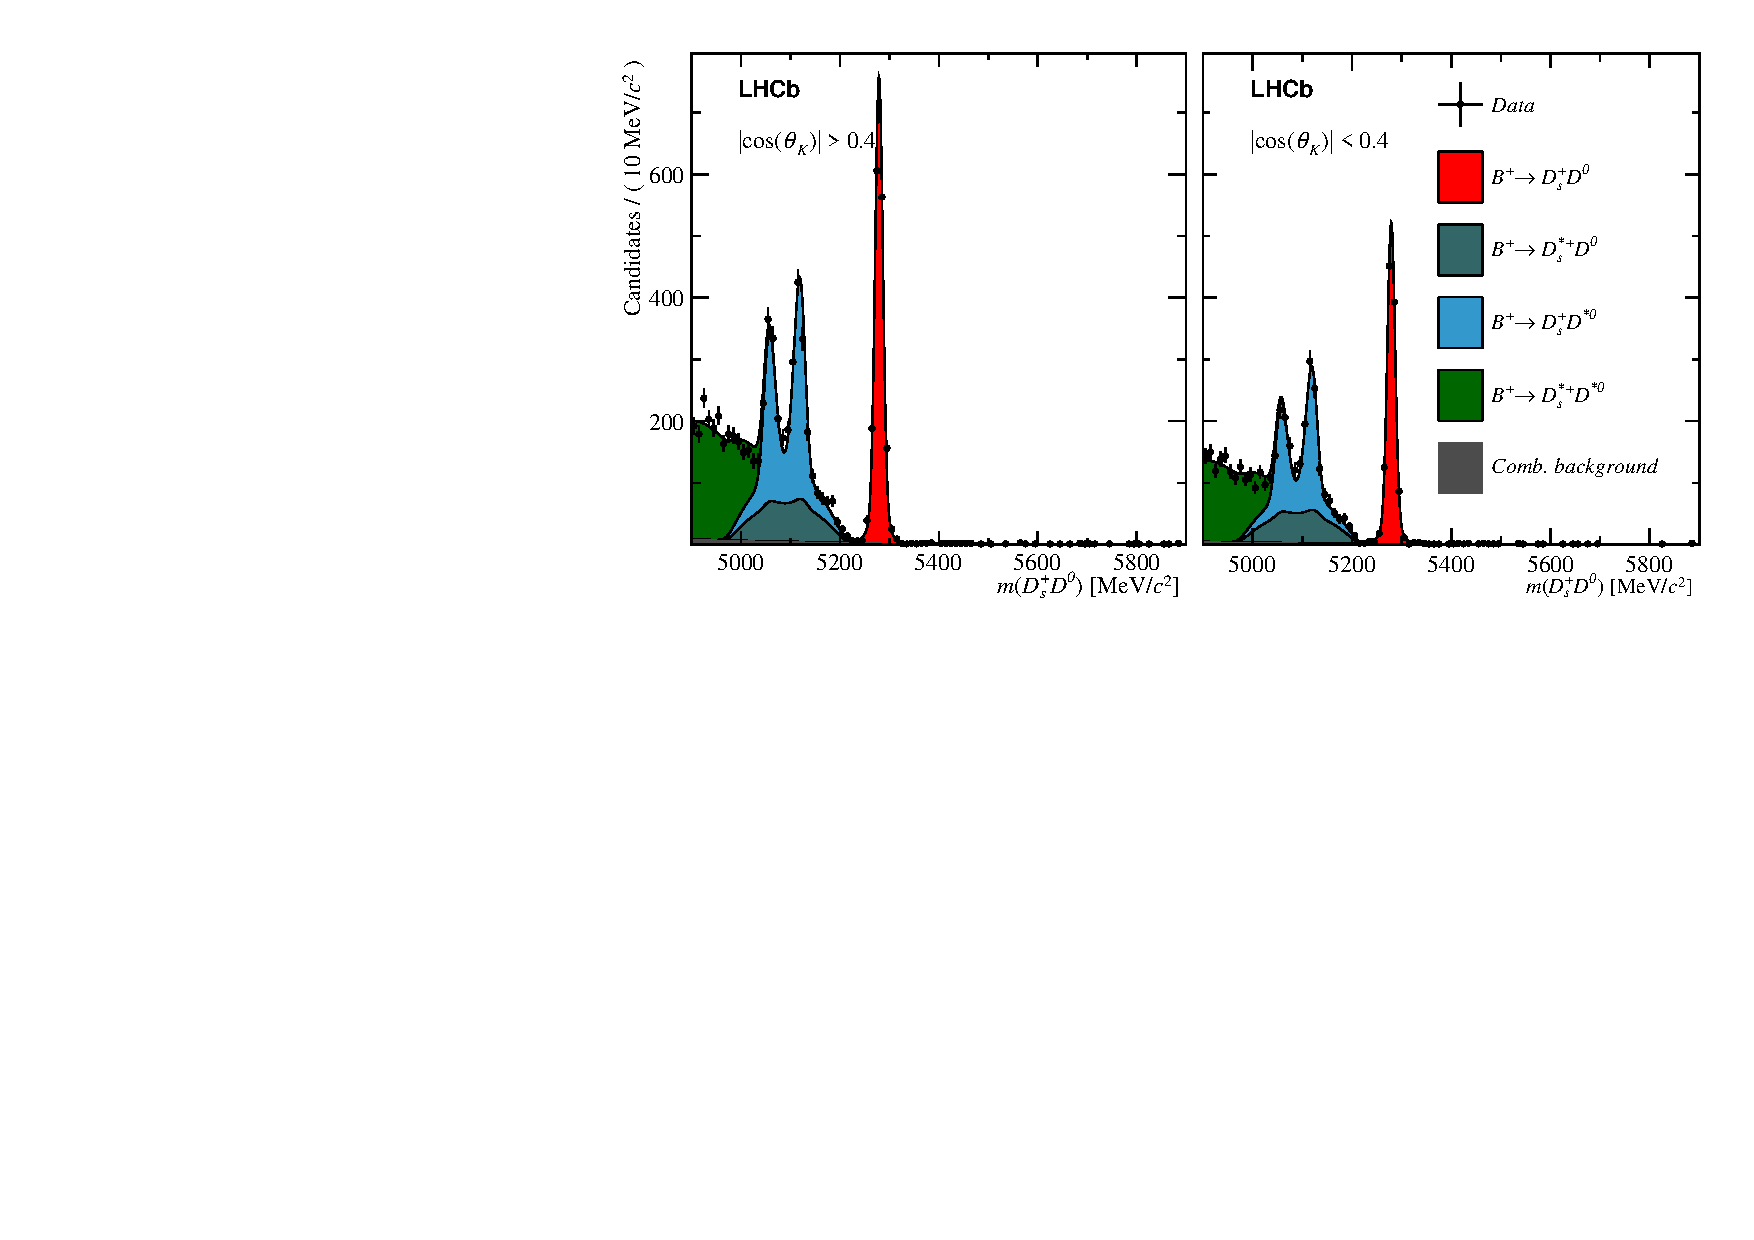
\includegraphics[width=0.7\textwidth]{figs/Appendix_FitCategories/canvas_DsD0_merged_both_summed_splitHel_splitKKPi_s21_s21r1_s24_s26.pdf}\\
        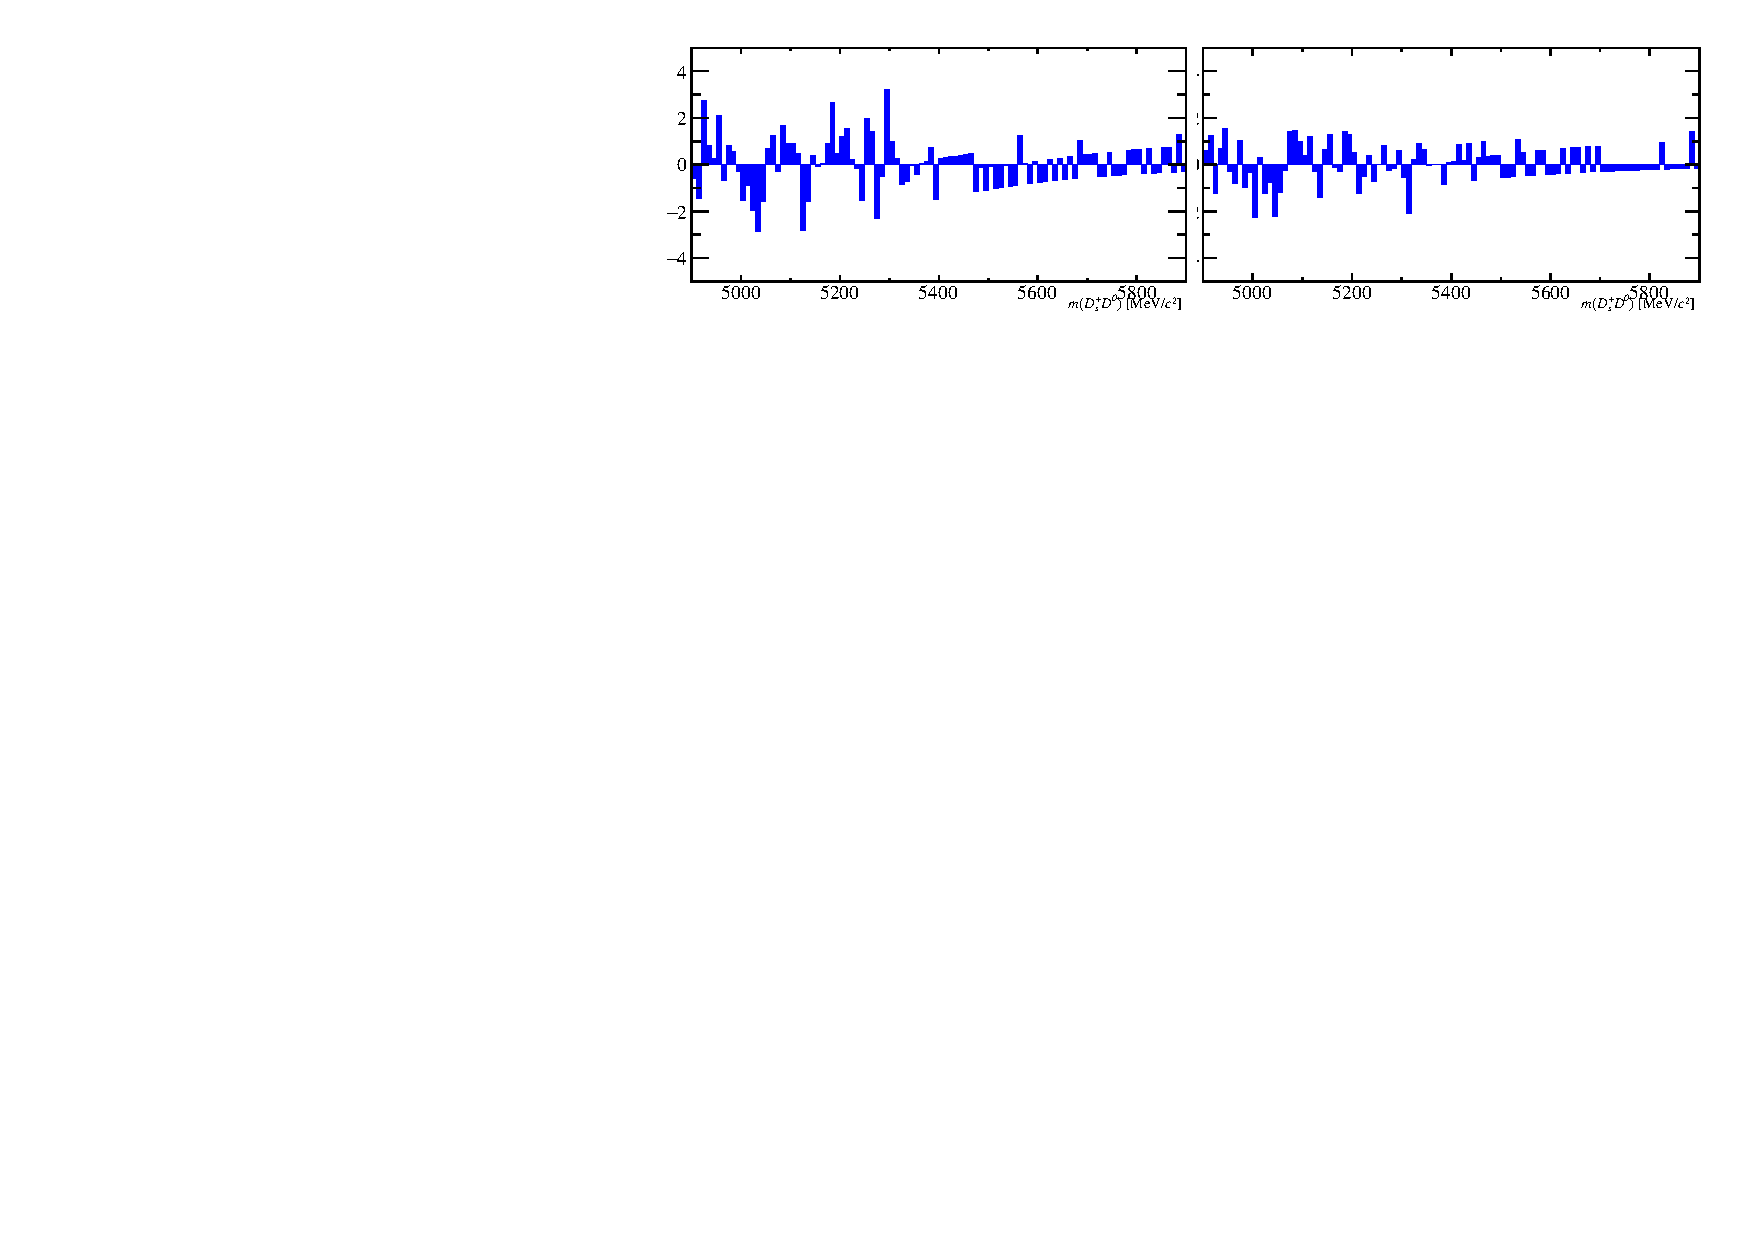
\includegraphics[width=0.7\textwidth]{figs/Appendix_FitCategories/residuals_DsD0_merged_both_summed_splitHel_splitKKPi_s21_s21r1_s24_s26.pdf}
    \end{subfigure}
    \begin{subfigure}[t]{1.0\textwidth}
        \centering
        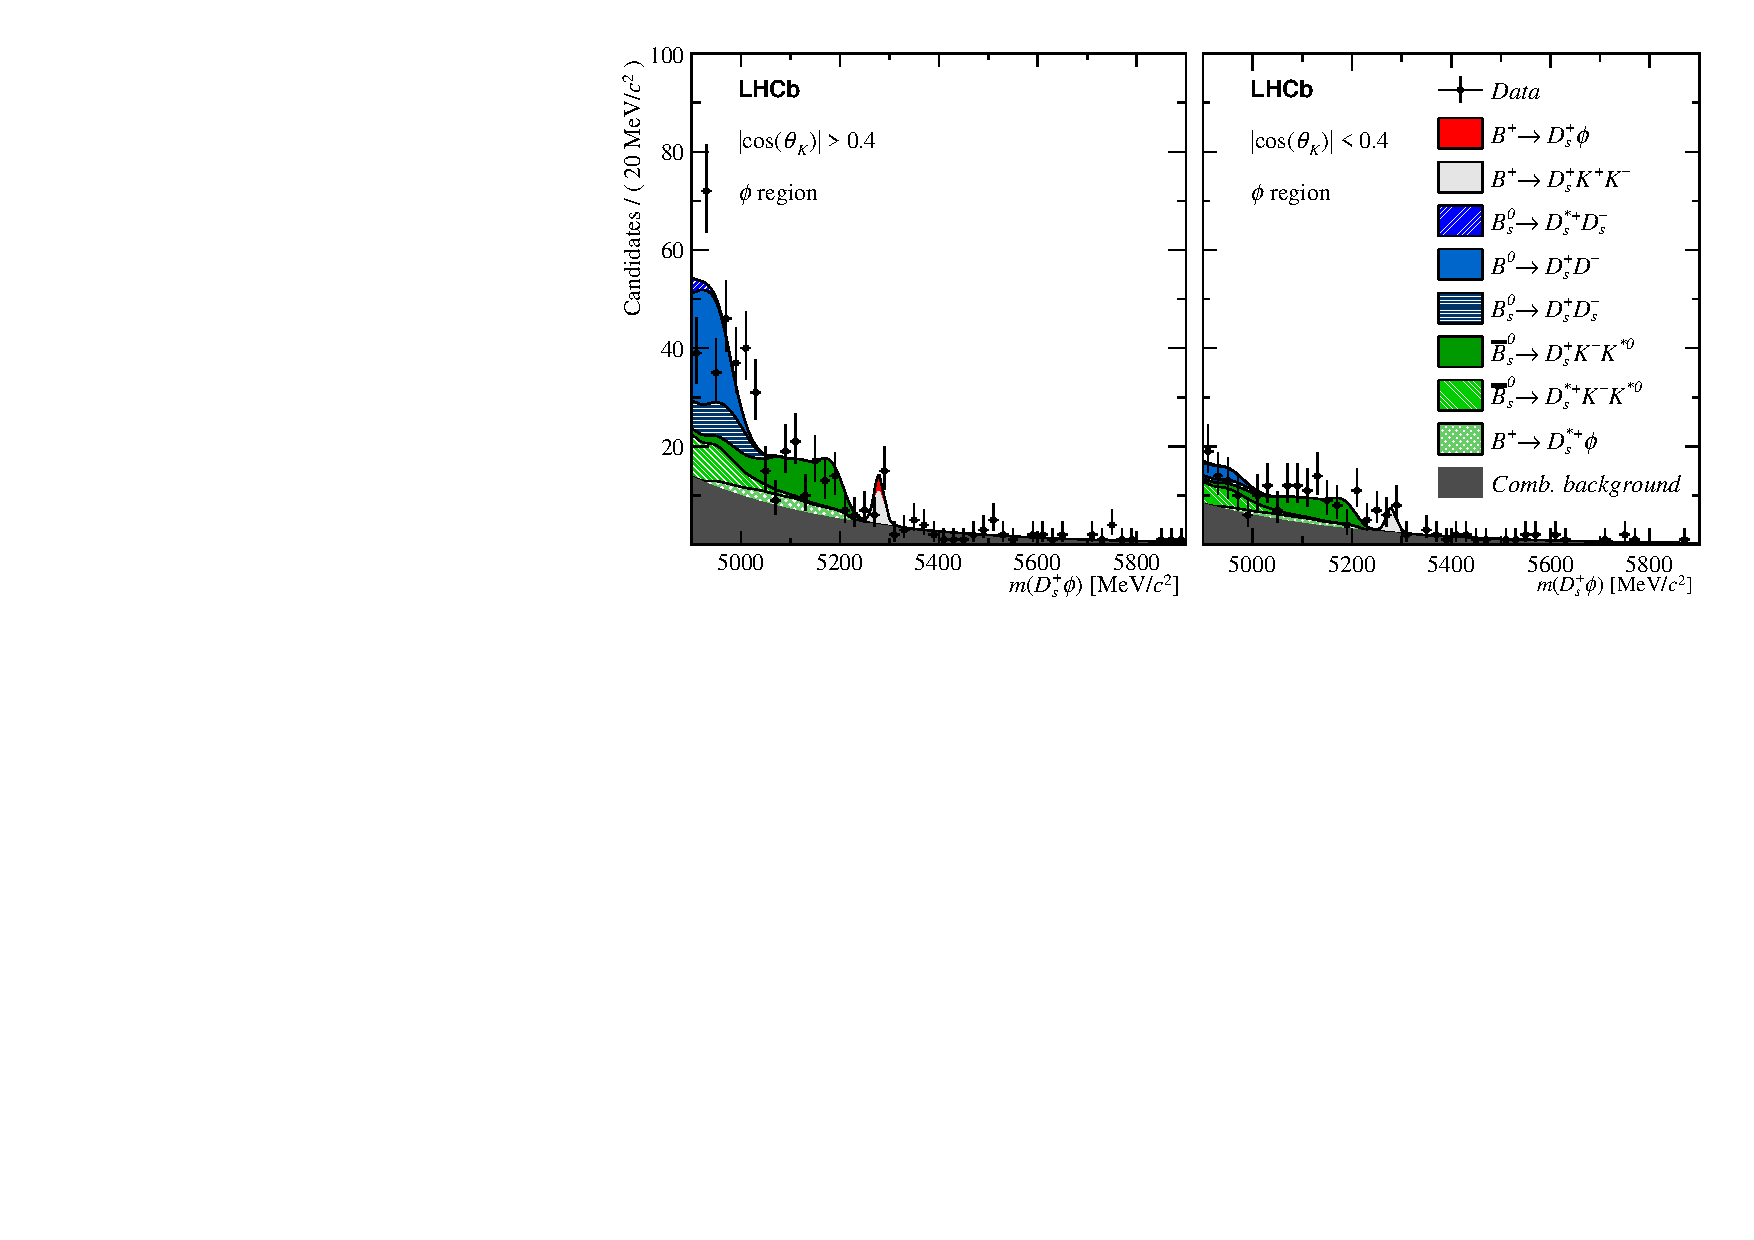
\includegraphics[width=0.7\textwidth]{figs/Appendix_FitCategories/canvas_DsPhi_merged_both_summed_splitHel_splitKKPi_s21_s21r1_s24_s26.pdf}\\
        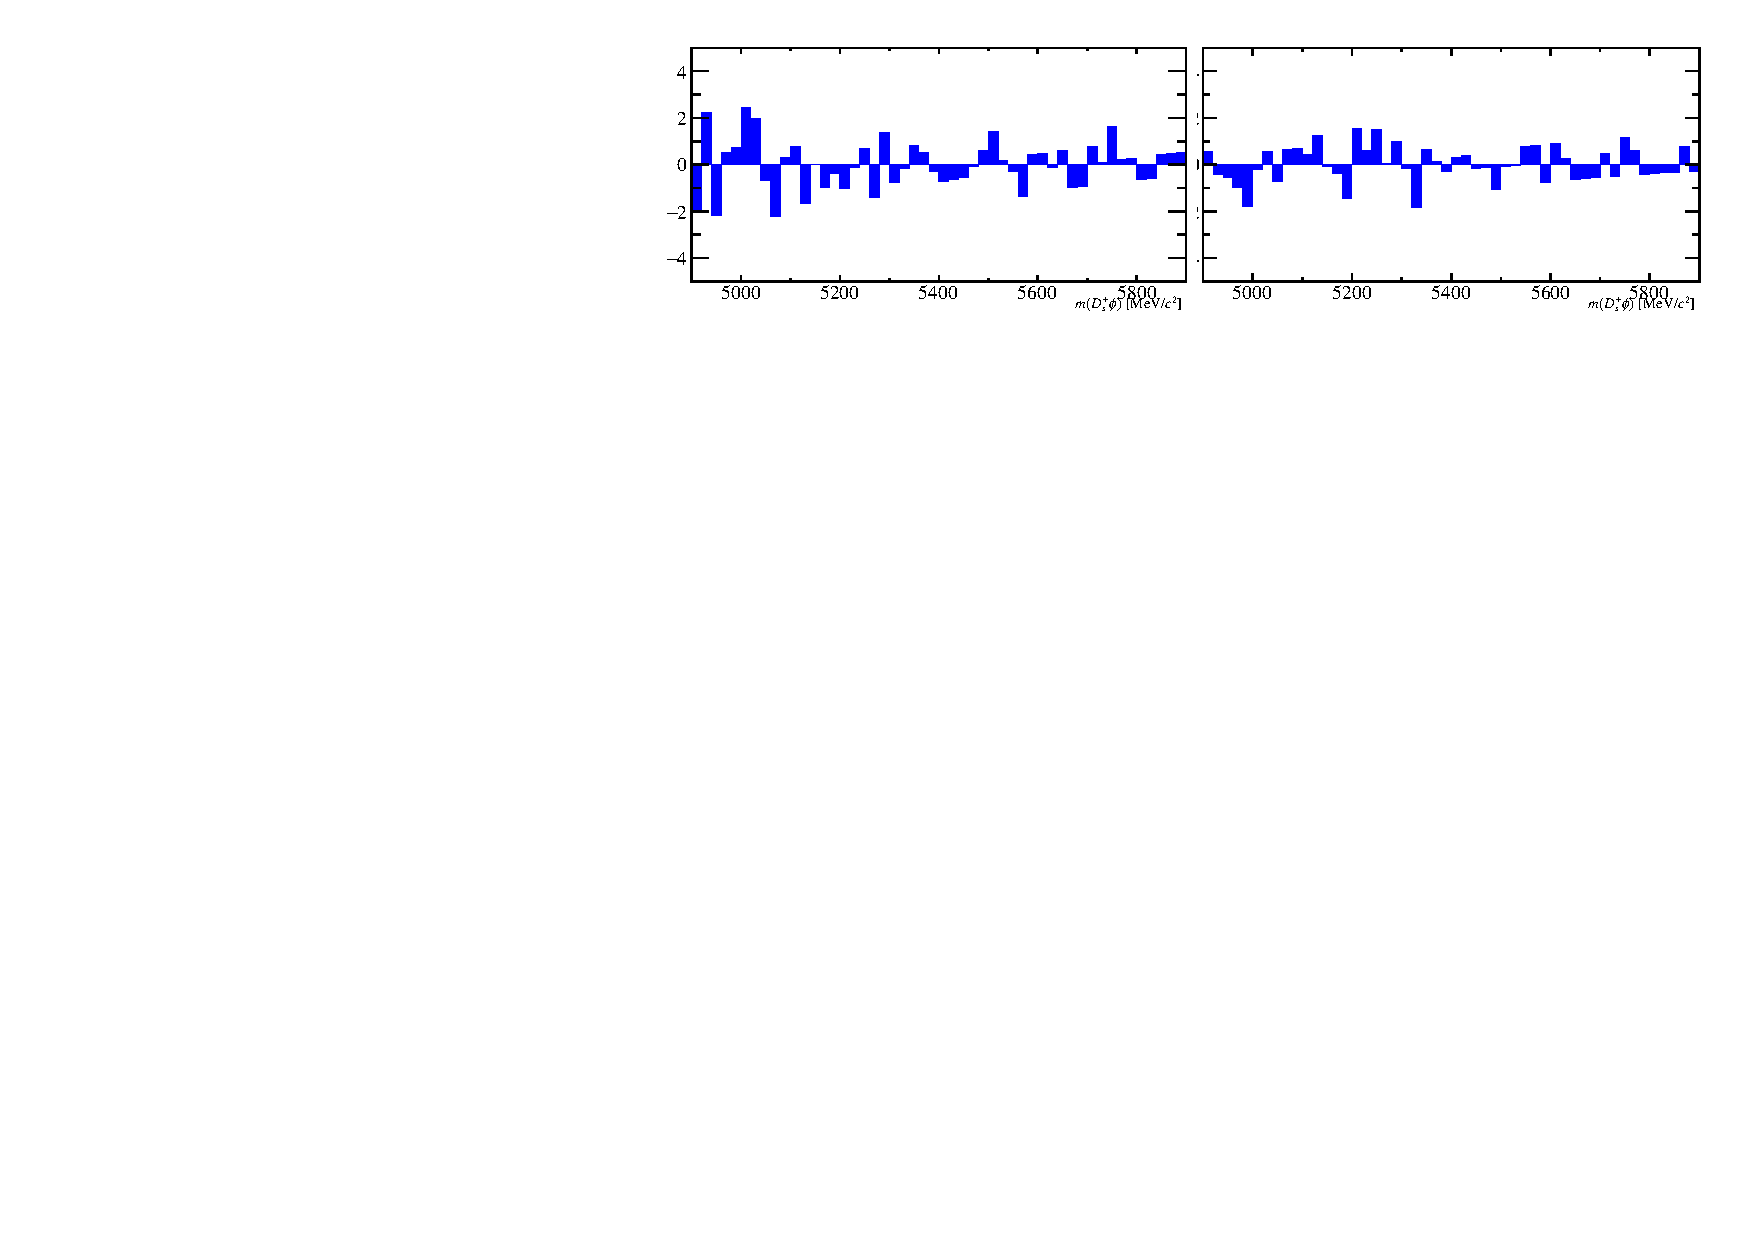
\includegraphics[width=0.7\textwidth]{figs/Appendix_FitCategories/residuals_DsPhi_merged_both_summed_splitHel_splitKKPi_s21_s21r1_s24_s26.pdf}
    \end{subfigure}
    \begin{subfigure}[t]{1.0\textwidth}
        \centering
        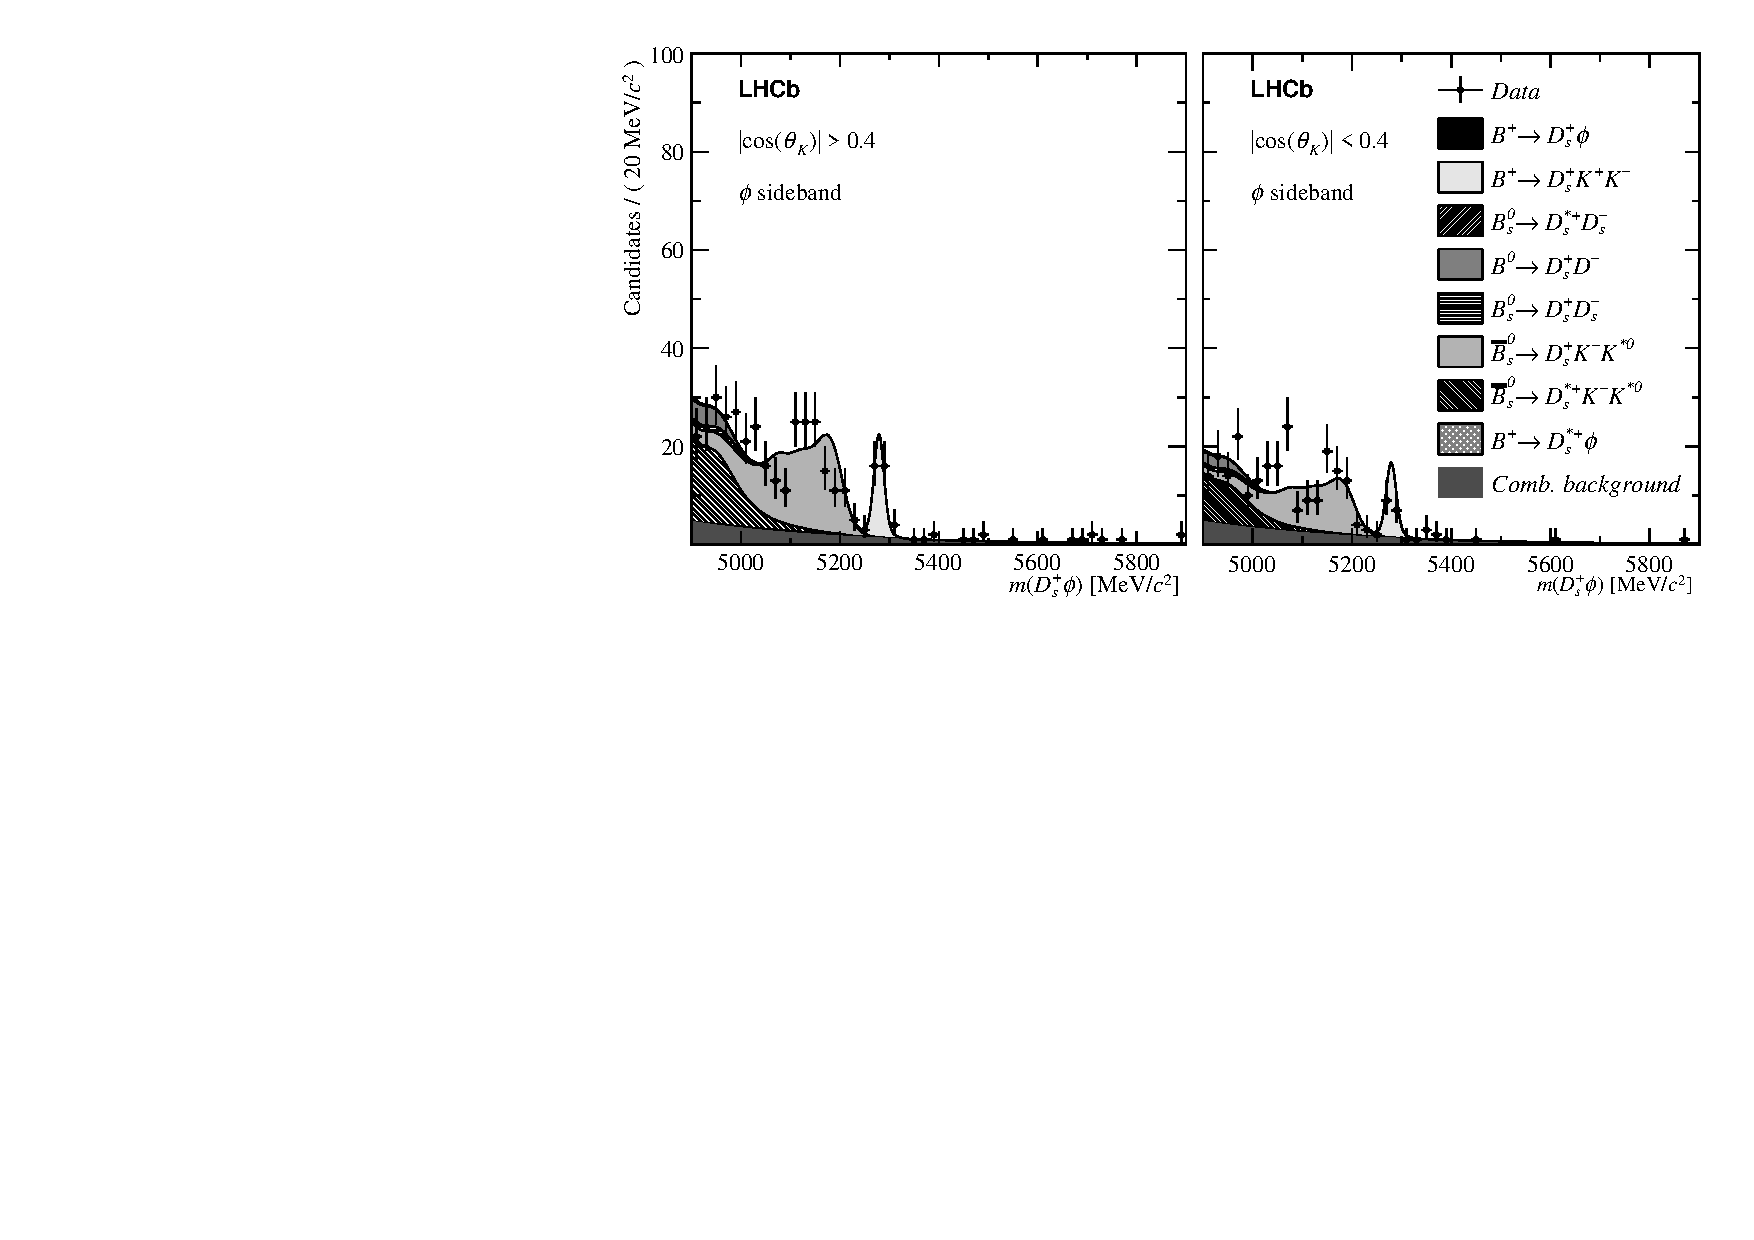
\includegraphics[width=0.7\textwidth]{figs/Appendix_FitCategories/canvas_DsPhiSide_merged_both_summed_splitHel_splitKKPi_s21_s21r1_s24_s26.pdf}\\
        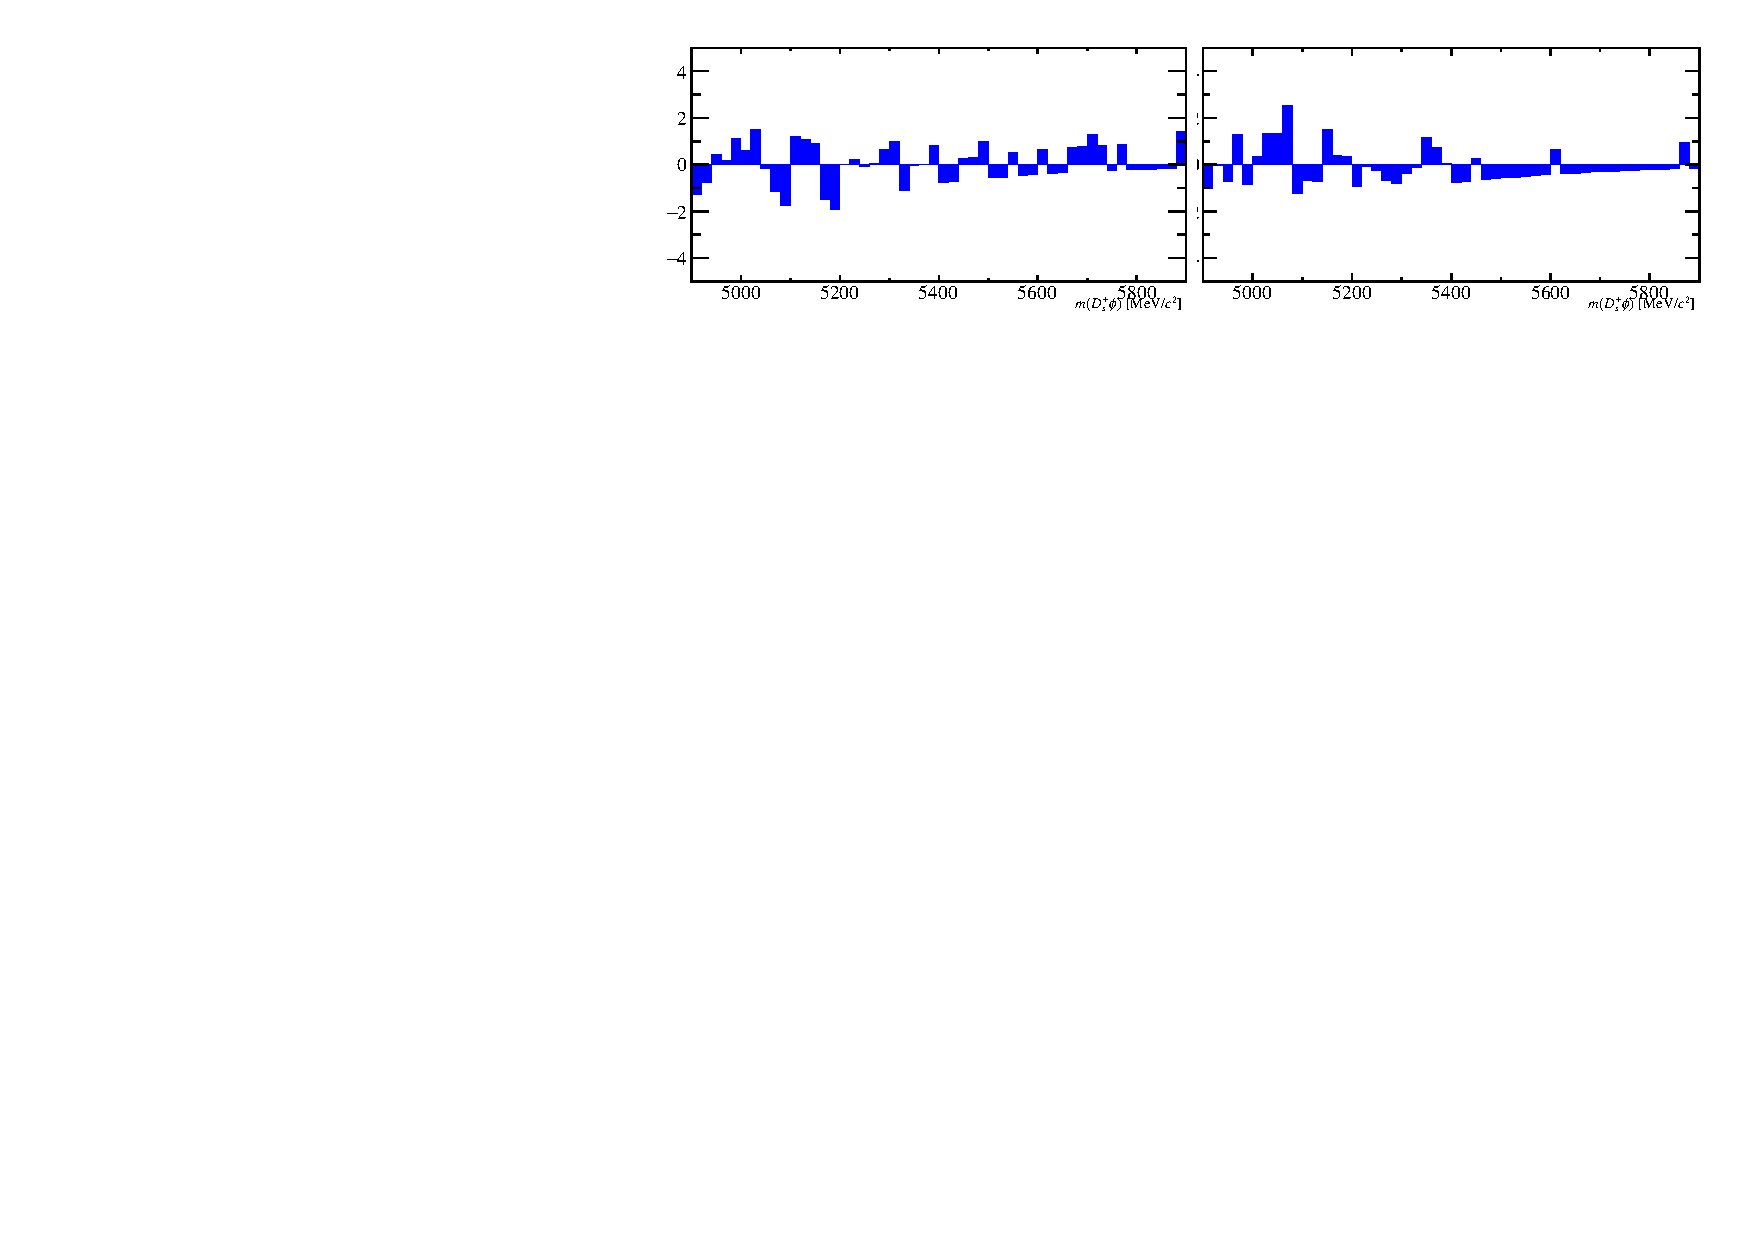
\includegraphics[width=0.7\textwidth]{figs/Appendix_FitCategories/residuals_DsPhiSide_merged_both_summed_splitHel_splitKKPi_s21_s21r1_s24_s26.pdf}
    \end{subfigure}
    \caption{Invariant mass fits to all \decay{\Bp}{\Dsp\phiz} candidates}
\end{figure}
%%%%%%%%%%%%%%%%%%%%%%%%%%%%%%%%%%%%%%%%%%%%%%%%%%%%%%%%%%




%%%%%%%%%%%%%%%%%%%%%%%%%%%%%%%%%%%%%%%%%%%%%%%%%%%%%%%%%%
\begin{figure}[!h]
    \centering
    \begin{subfigure}[t]{1.0\textwidth}
        \centering
        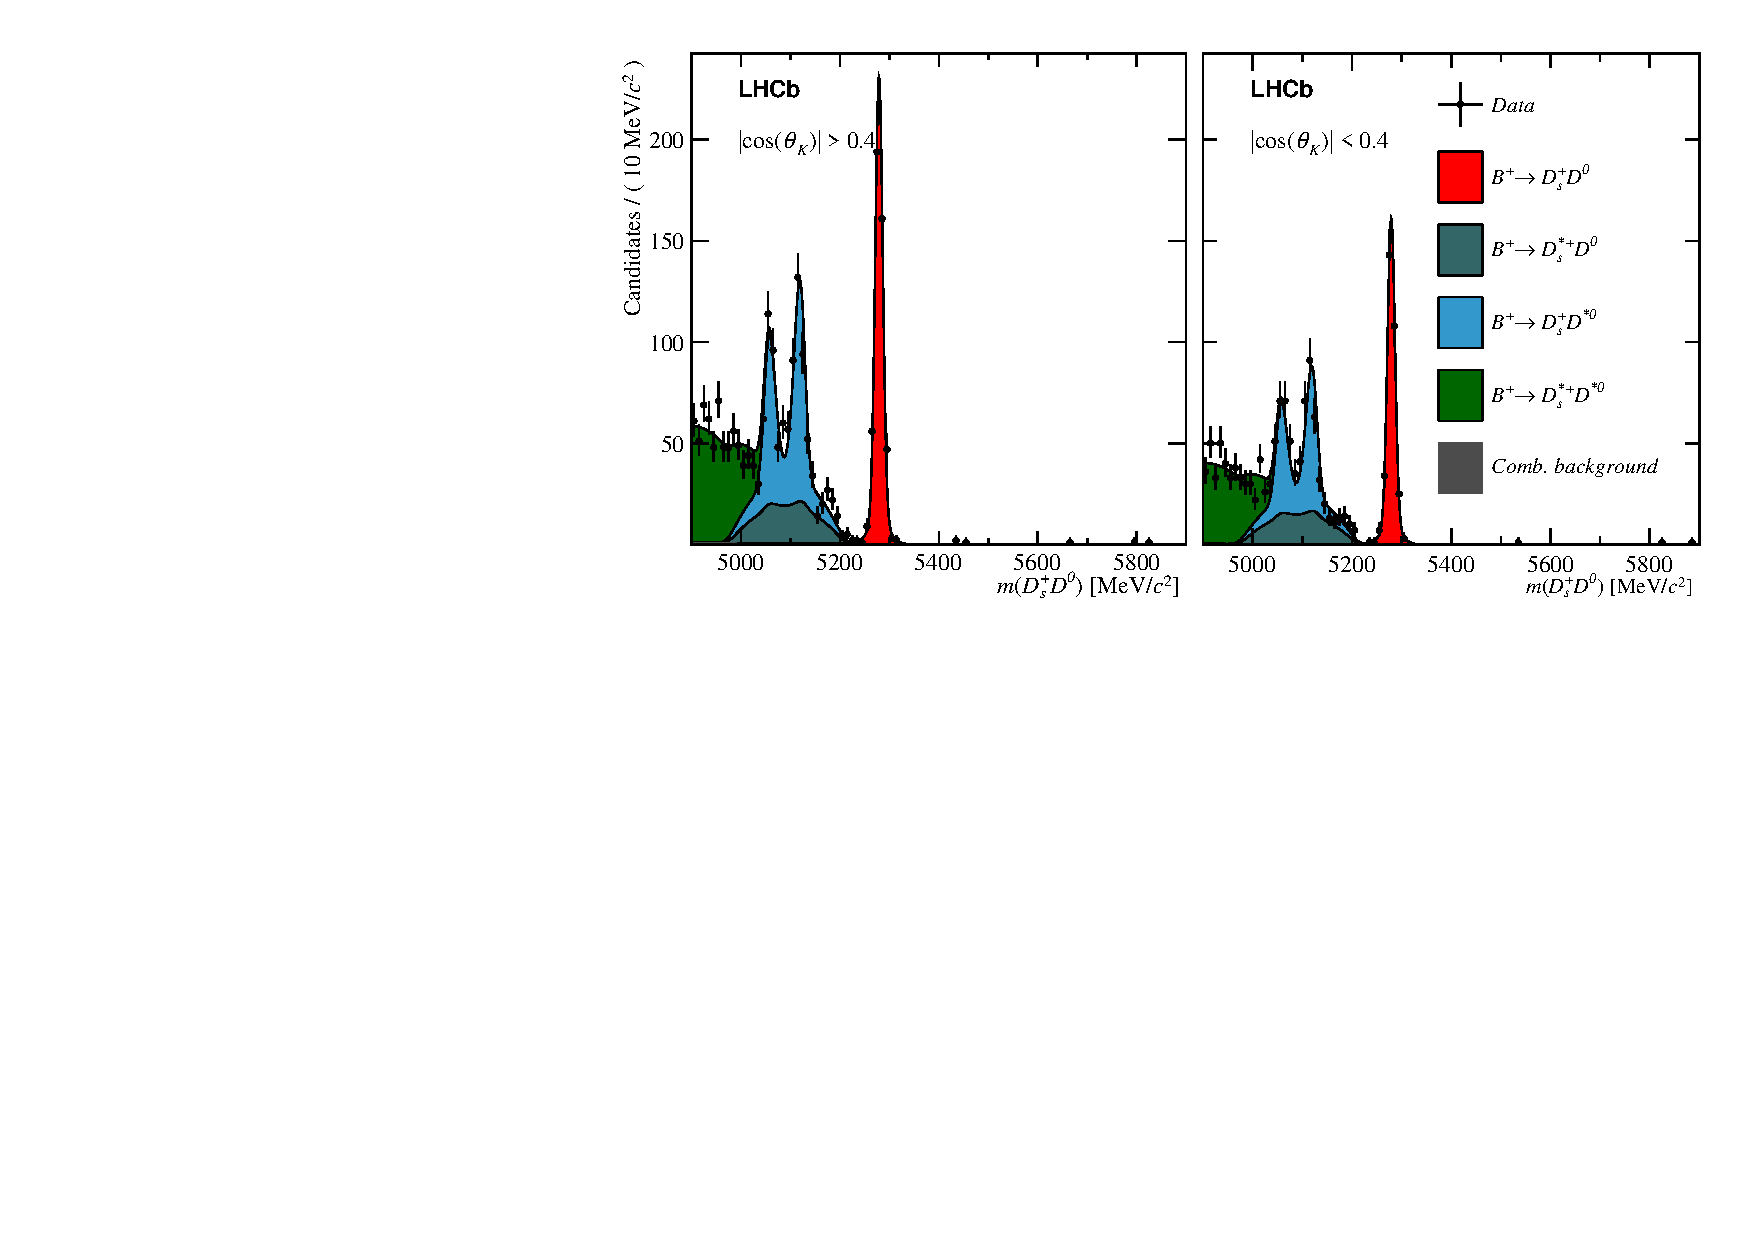
\includegraphics[width=0.7\textwidth]{figs/Appendix_FitCategories/canvas_DsD0_Ds2PhiPi_both_summed_splitHel_splitKKPi_s21_s21r1_s24_s26.pdf}\\
        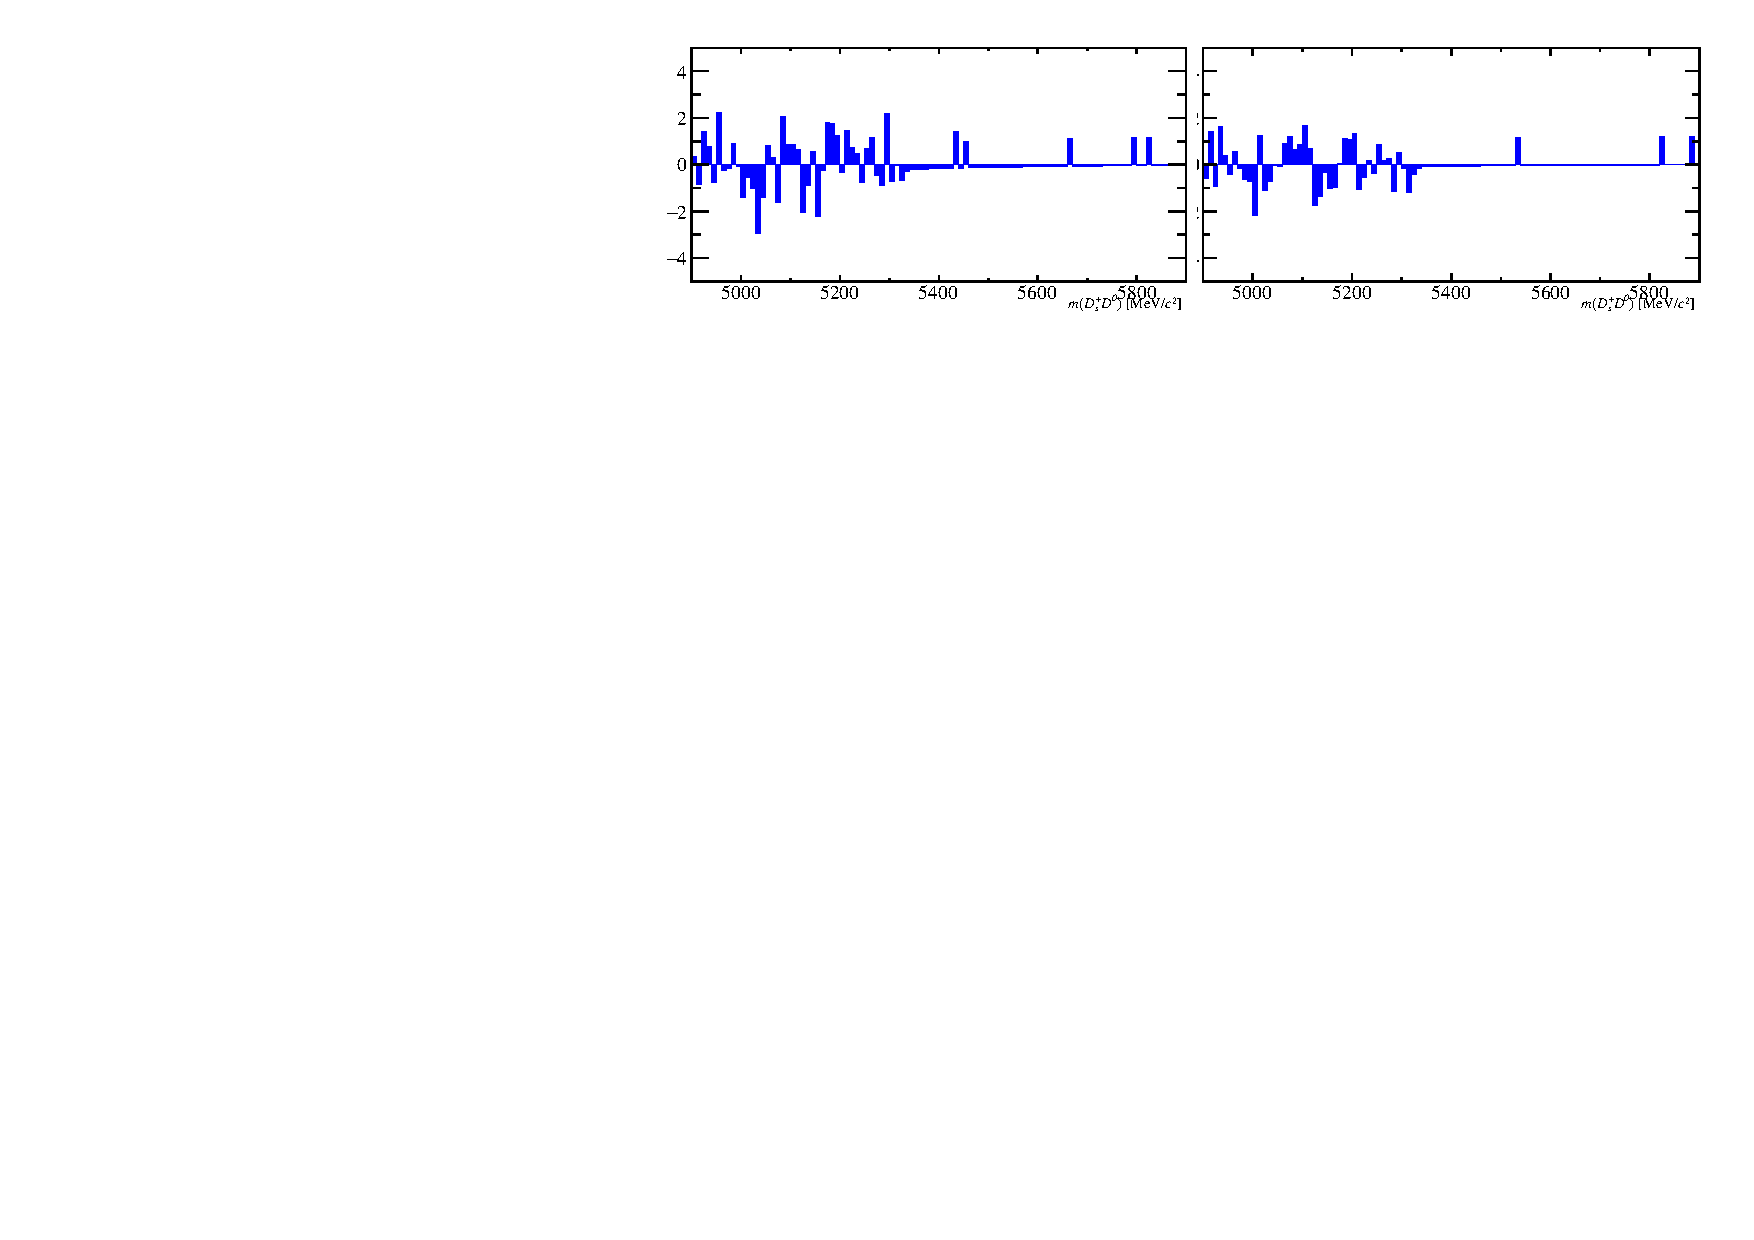
\includegraphics[width=0.7\textwidth]{figs/Appendix_FitCategories/residuals_DsD0_Ds2PhiPi_both_summed_splitHel_splitKKPi_s21_s21r1_s24_s26.pdf}
    \end{subfigure}
    \begin{subfigure}[t]{1.0\textwidth}
        \centering
        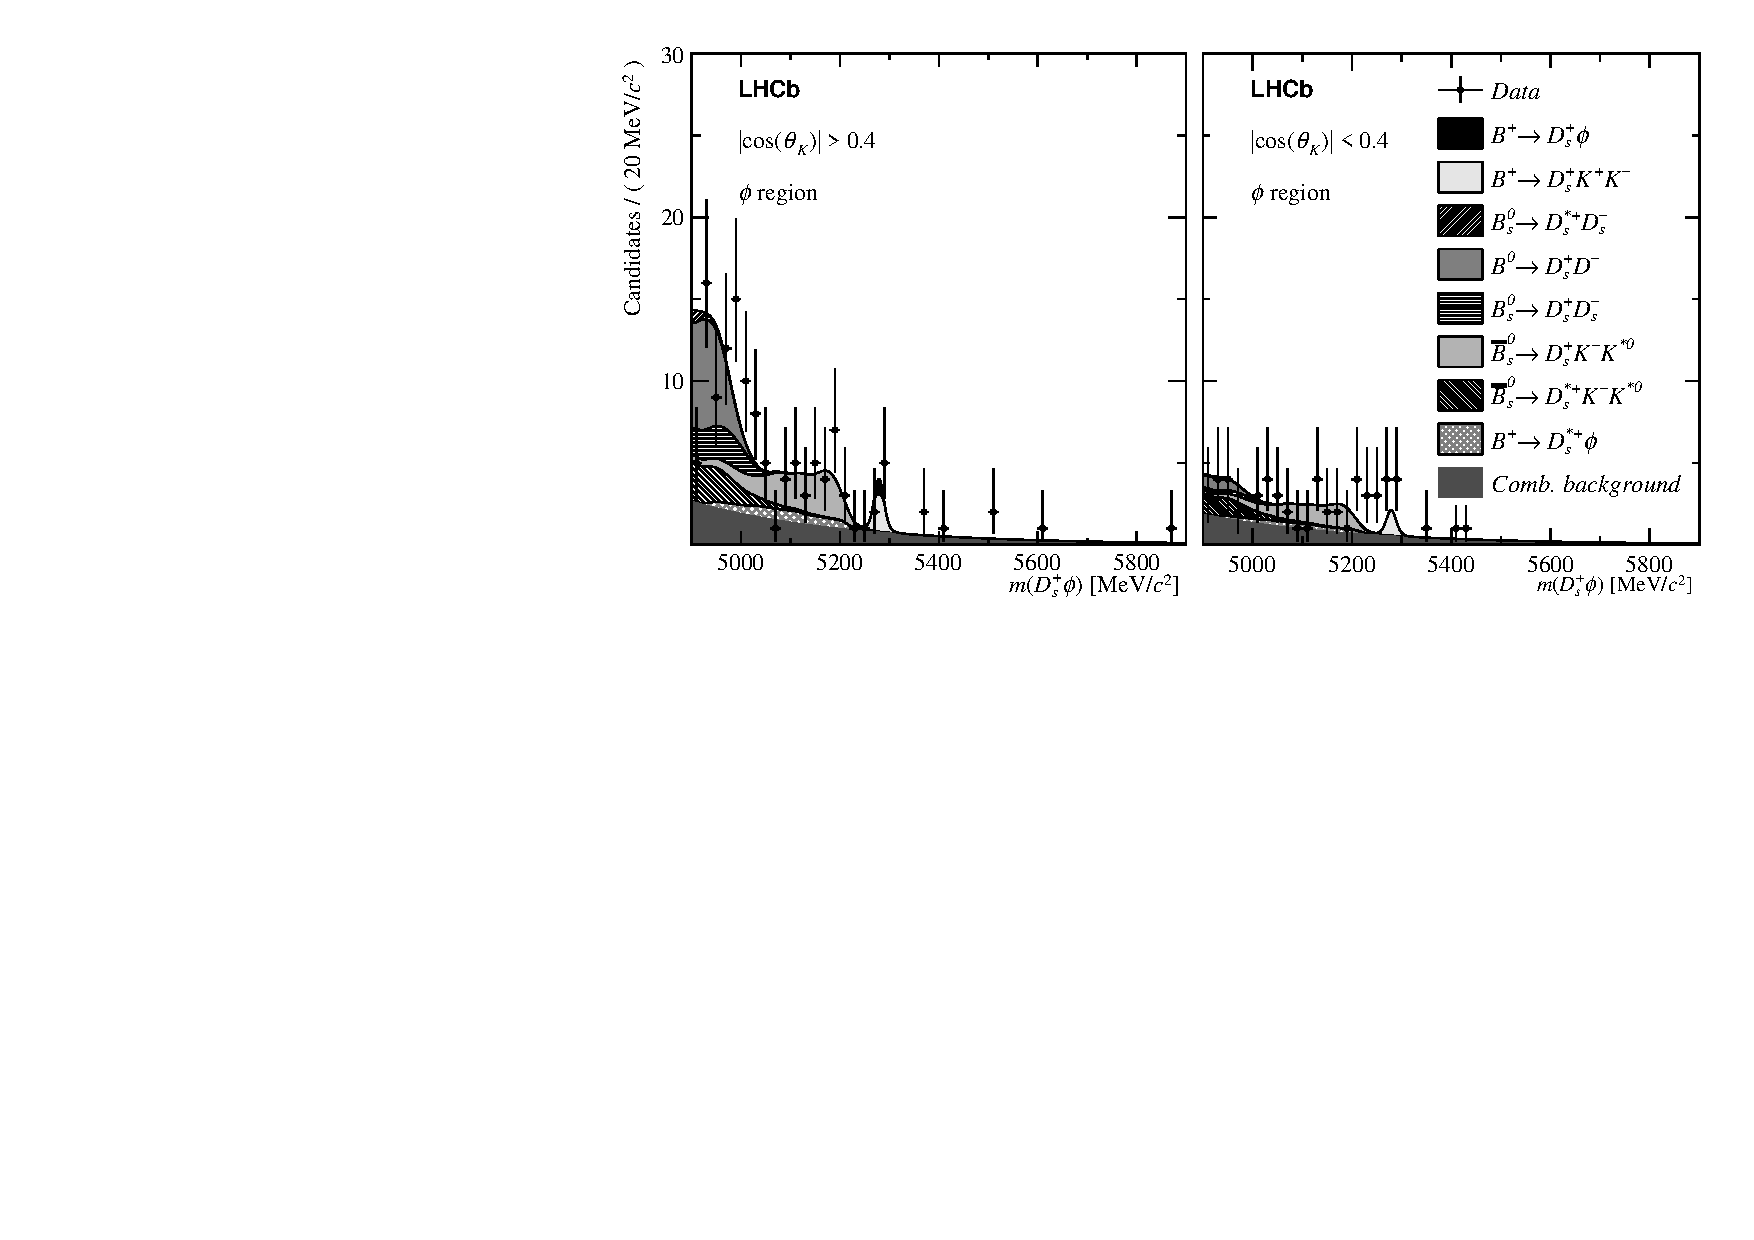
\includegraphics[width=0.7\textwidth]{figs/Appendix_FitCategories/canvas_DsPhi_Ds2PhiPi_both_summed_splitHel_splitKKPi_s21_s21r1_s24_s26.pdf}\\
        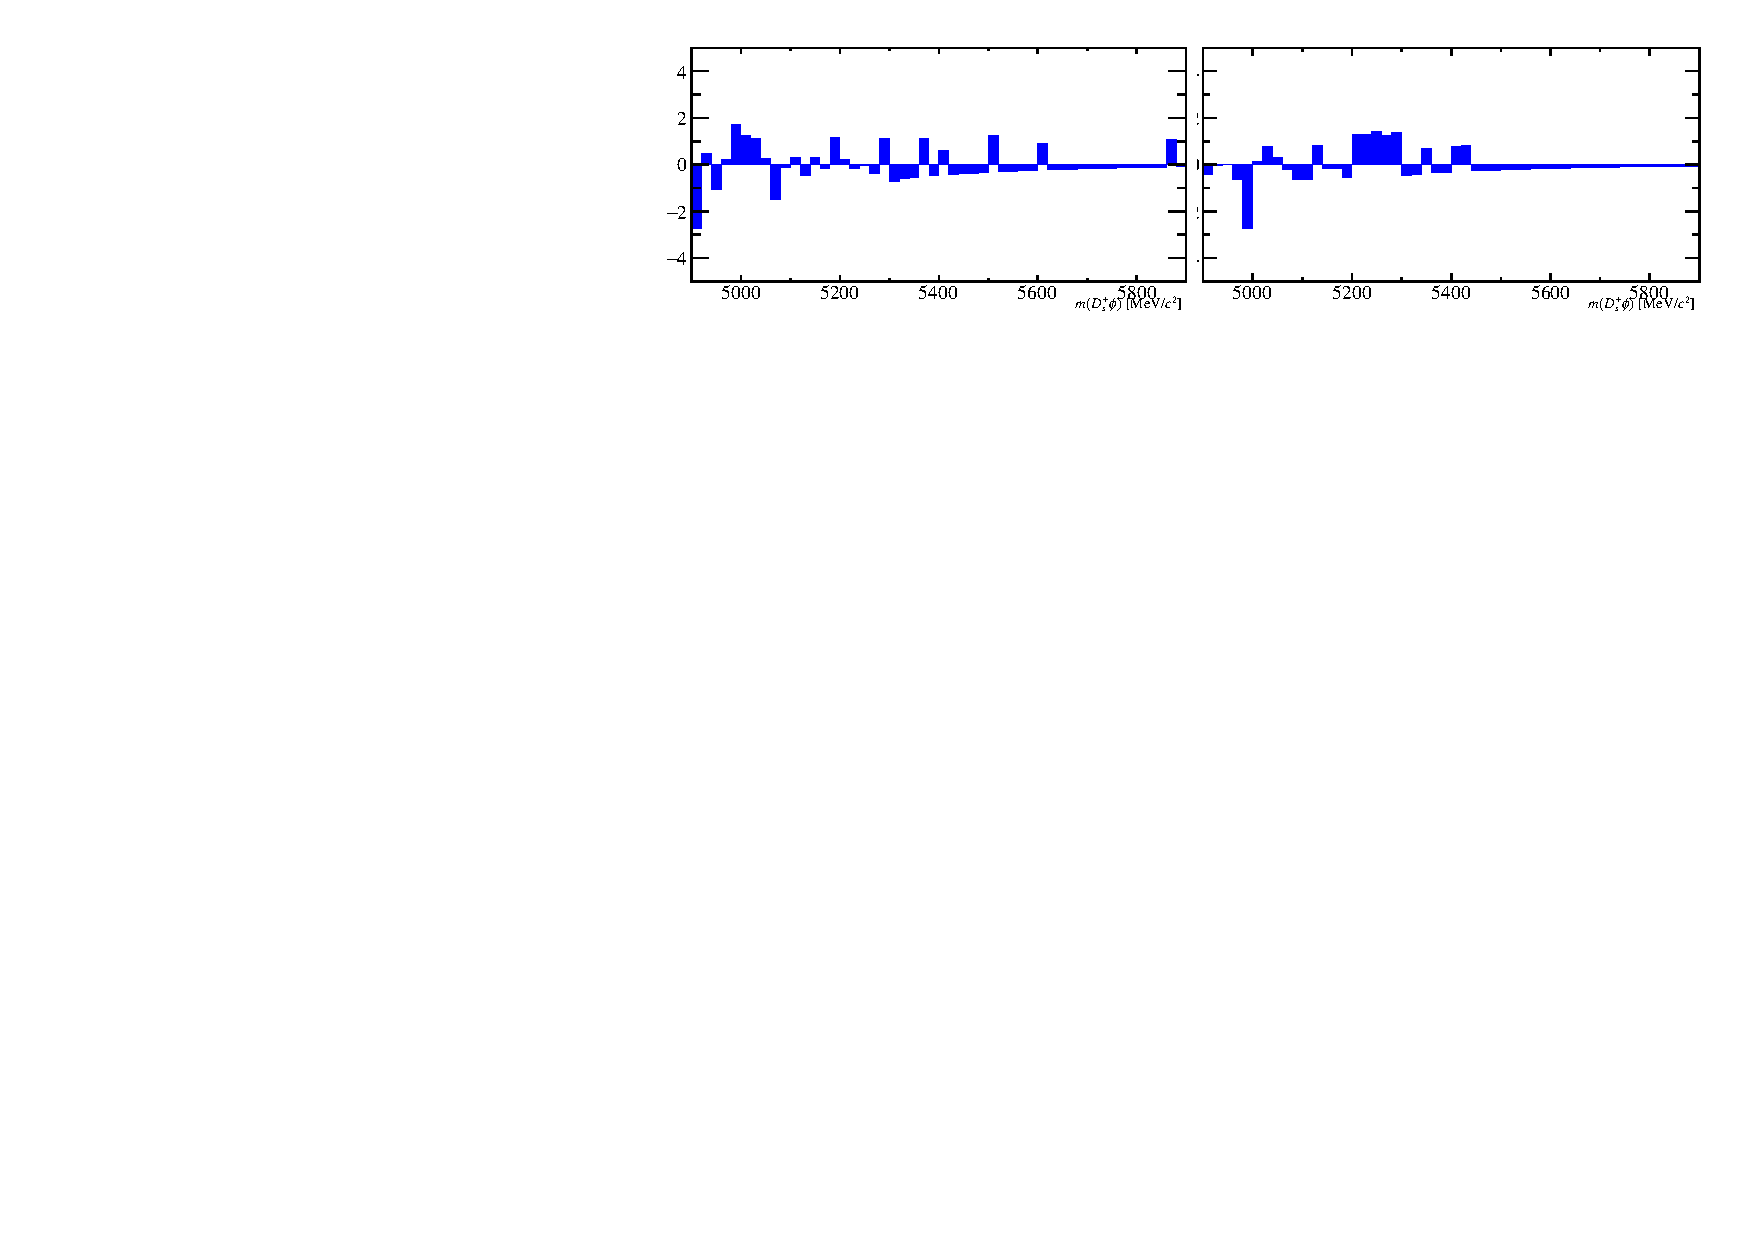
\includegraphics[width=0.7\textwidth]{figs/Appendix_FitCategories/residuals_DsPhi_Ds2PhiPi_both_summed_splitHel_splitKKPi_s21_s21r1_s24_s26.pdf}
    \end{subfigure}
    \begin{subfigure}[t]{1.0\textwidth}
        \centering
        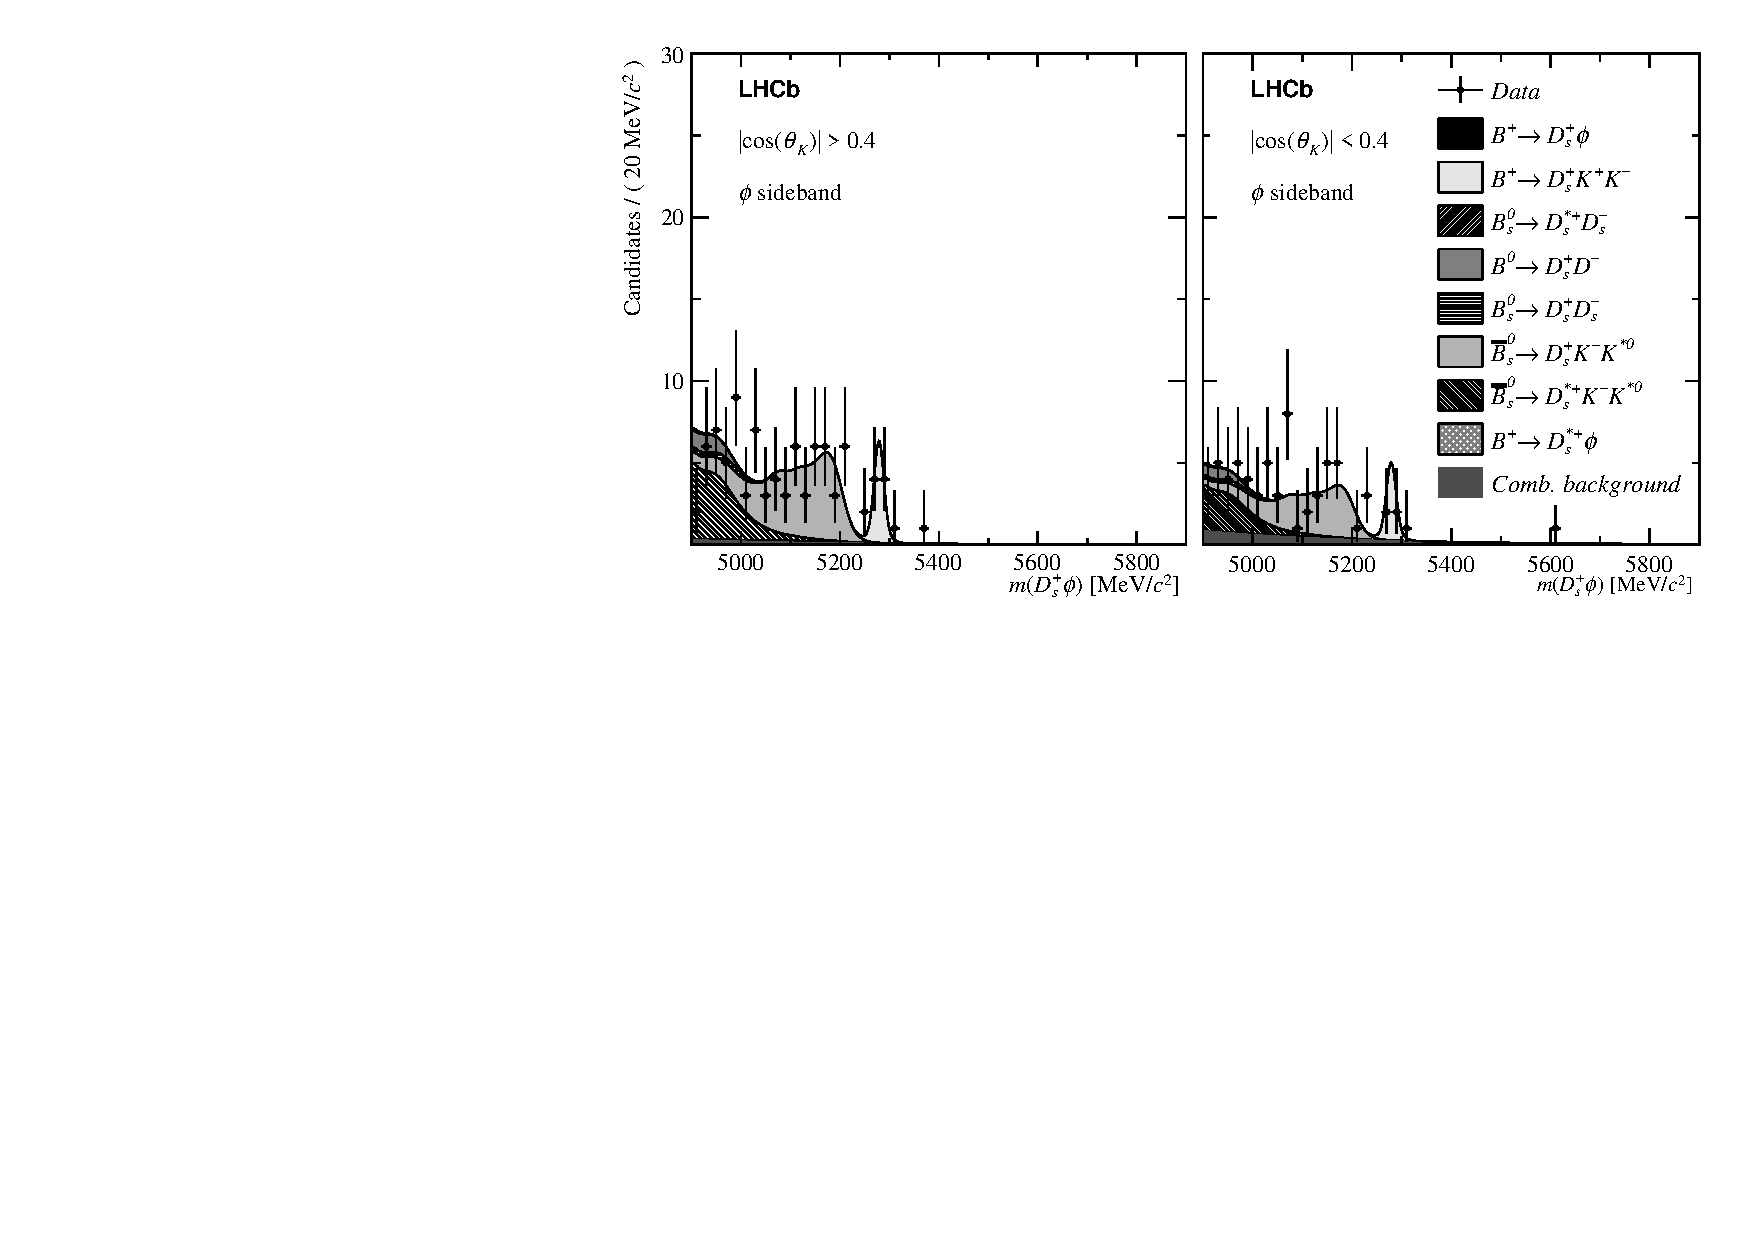
\includegraphics[width=0.7\textwidth]{figs/Appendix_FitCategories/canvas_DsPhiSide_Ds2PhiPi_both_summed_splitHel_splitKKPi_s21_s21r1_s24_s26.pdf}\\
        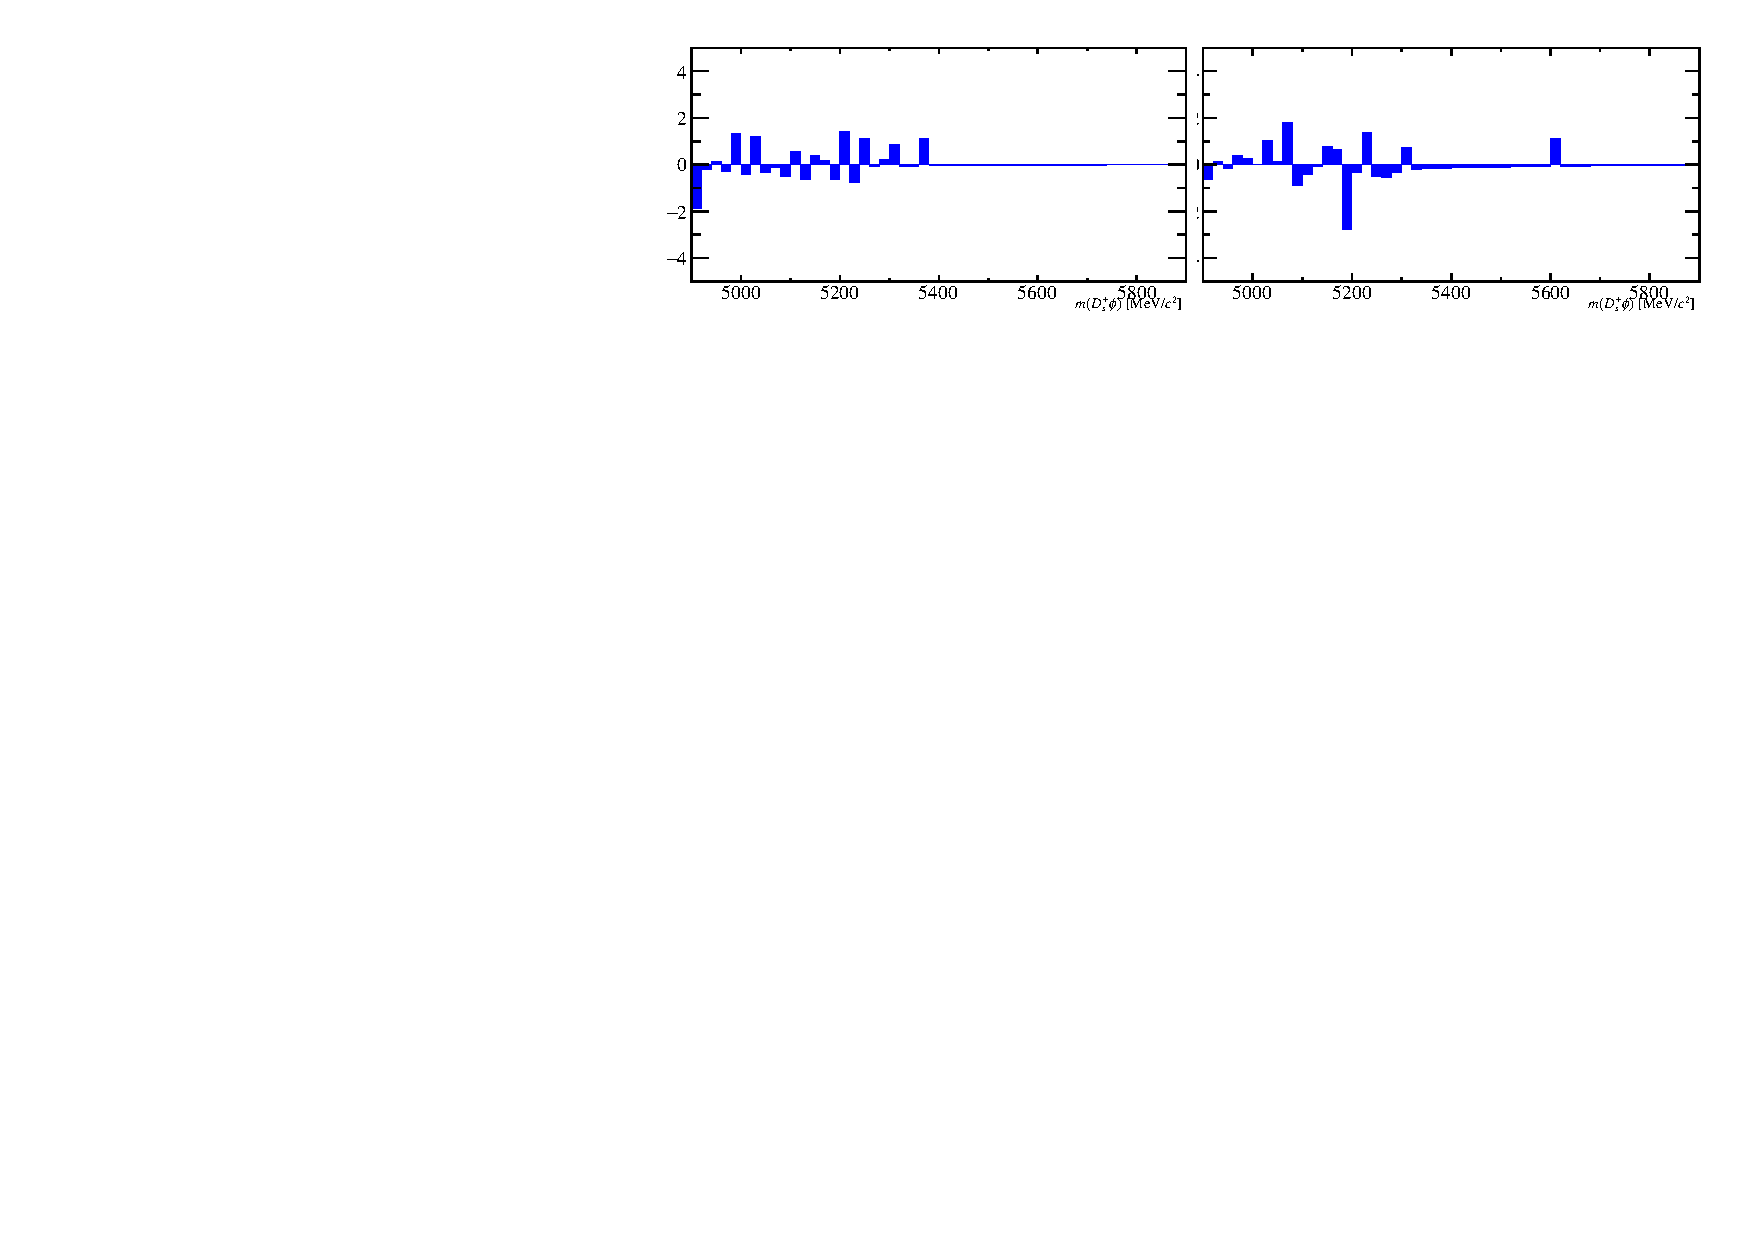
\includegraphics[width=0.7\textwidth]{figs/Appendix_FitCategories/residuals_DsPhiSide_Ds2PhiPi_both_summed_splitHel_splitKKPi_s21_s21r1_s24_s26.pdf}
    \end{subfigure}
    \caption{Invariant mass fits to \decay{\Bp}{\Dsp\phiz} candidates with \decay{\Dsp}{\phiz\pip}.}
\end{figure}
%%%%%%%%%%%%%%%%%%%%%%%%%%%%%%%%%%%%%%%%%%%%%%%%%%%%%%%%%%

%%%%%%%%%%%%%%%%%%%%%%%%%%%%%%%%%%%%%%%%%%%%%%%%%%%%%%%%%%
\begin{figure}[!h]
    \centering
    \begin{subfigure}[t]{1.0\textwidth}
        \centering
        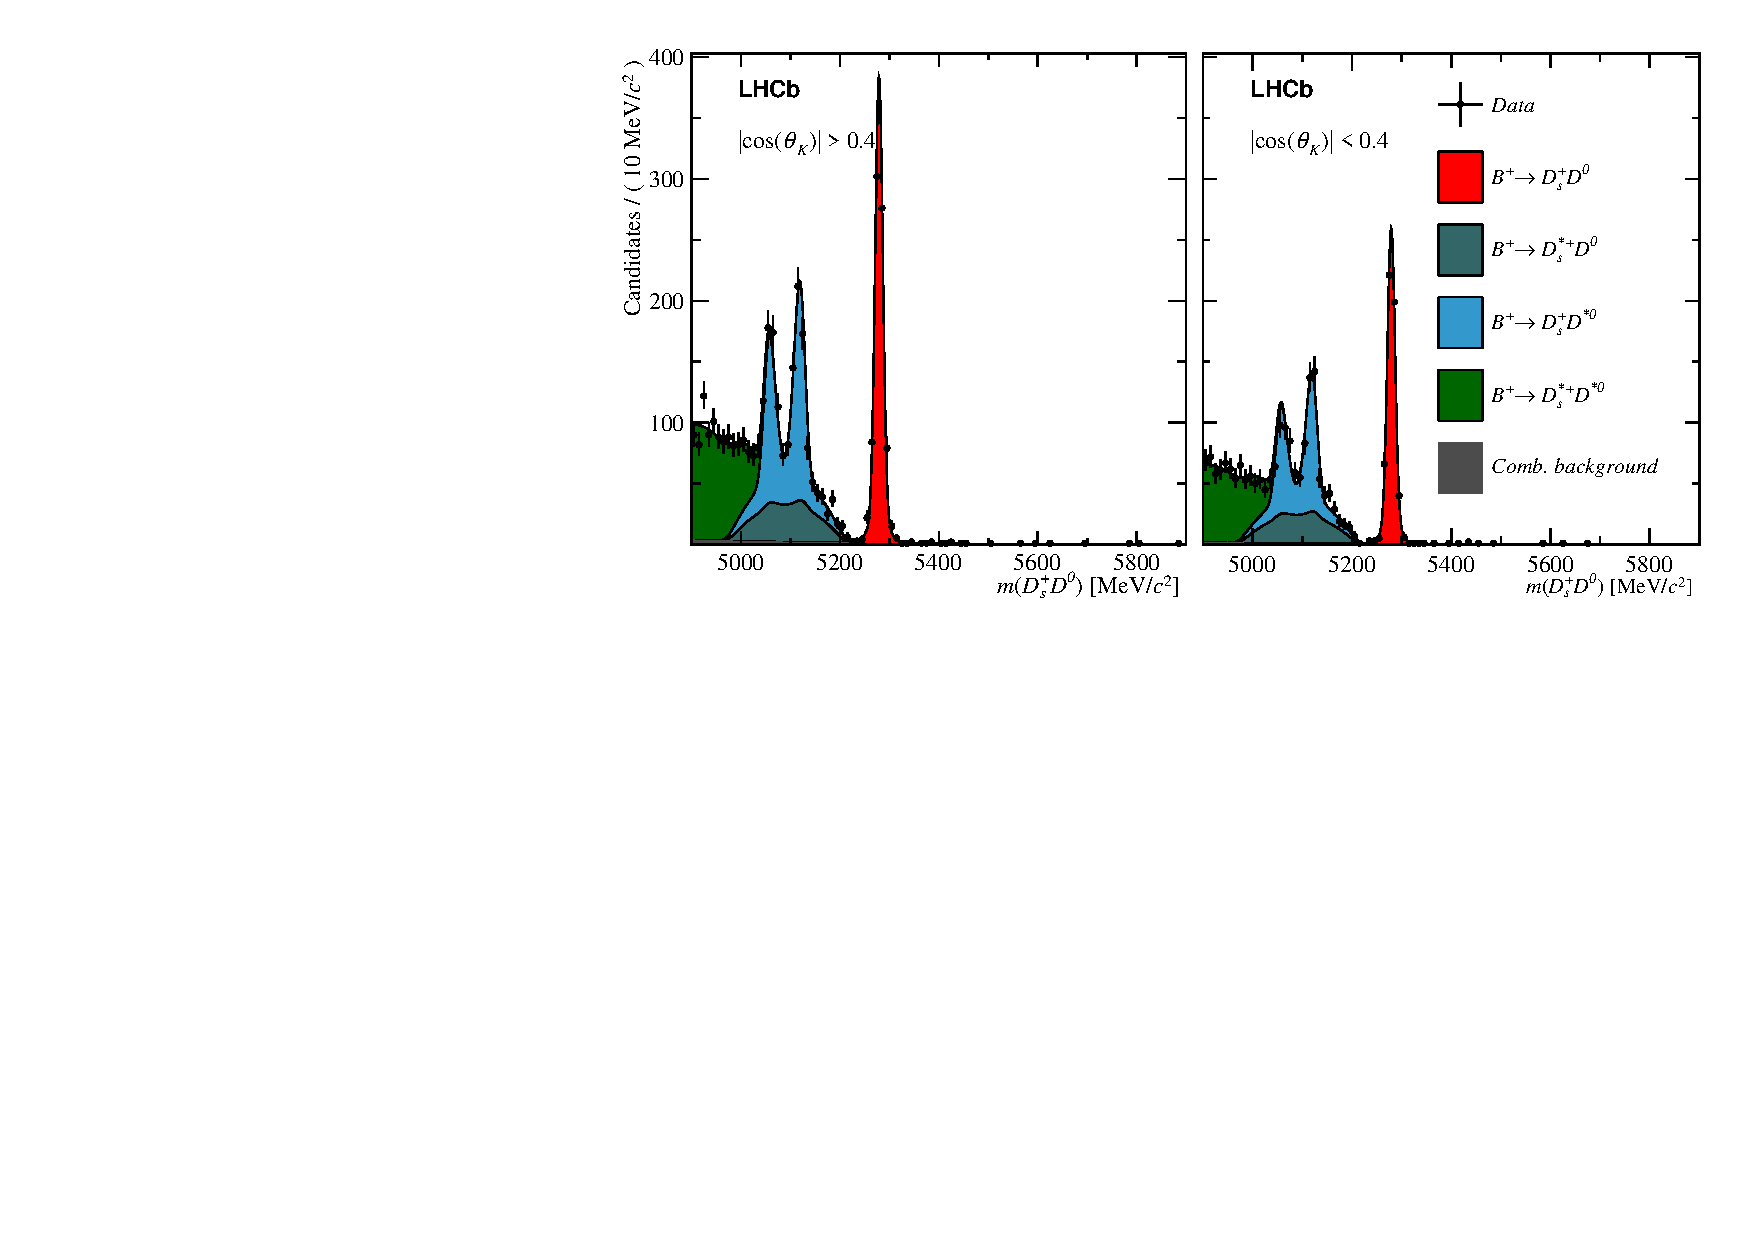
\includegraphics[width=0.7\textwidth]{figs/Appendix_FitCategories/canvas_DsD0_Ds2KKPi_both_summed_splitHel_splitKKPi_s21_s21r1_s24_s26.pdf}\\
        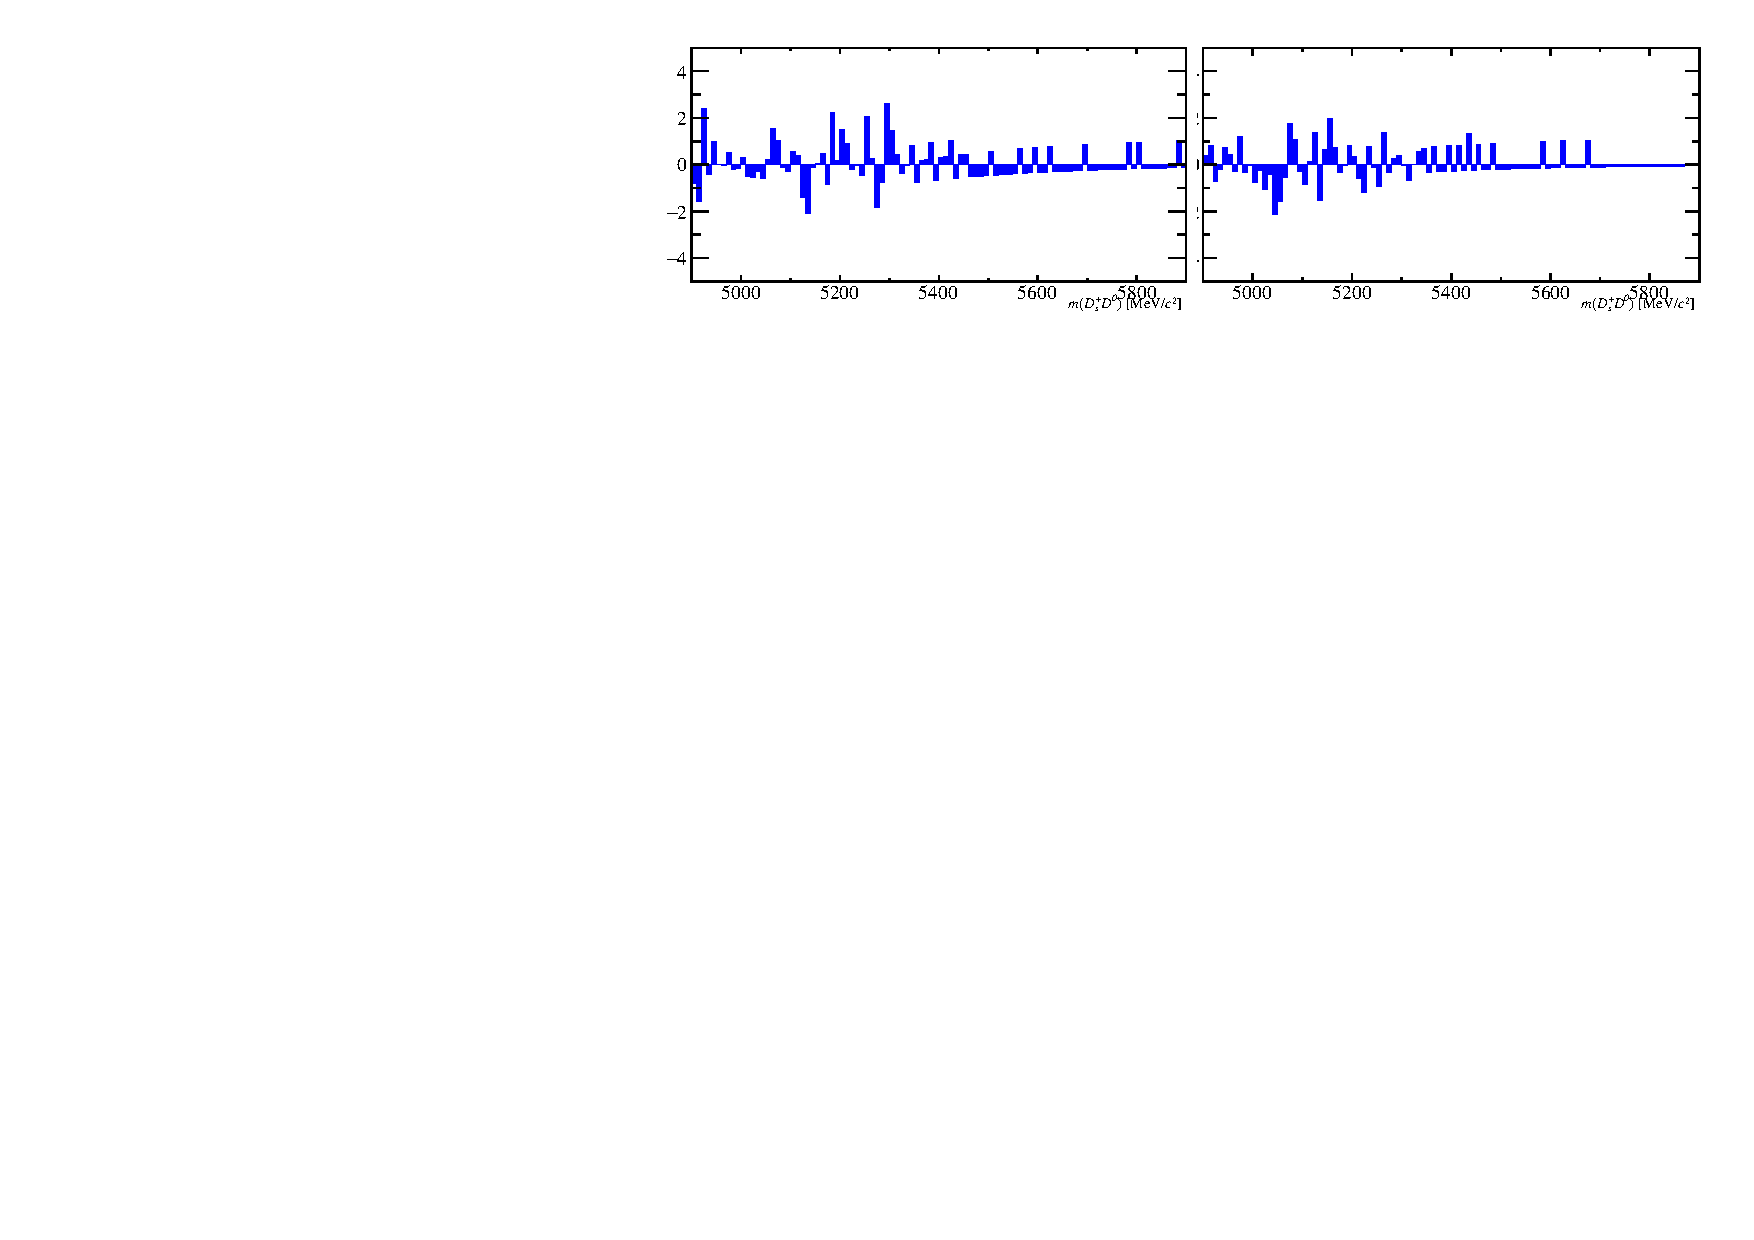
\includegraphics[width=0.7\textwidth]{figs/Appendix_FitCategories/residuals_DsD0_Ds2KKPi_both_summed_splitHel_splitKKPi_s21_s21r1_s24_s26.pdf}
    \end{subfigure}
    \begin{subfigure}[t]{1.0\textwidth}
        \centering
        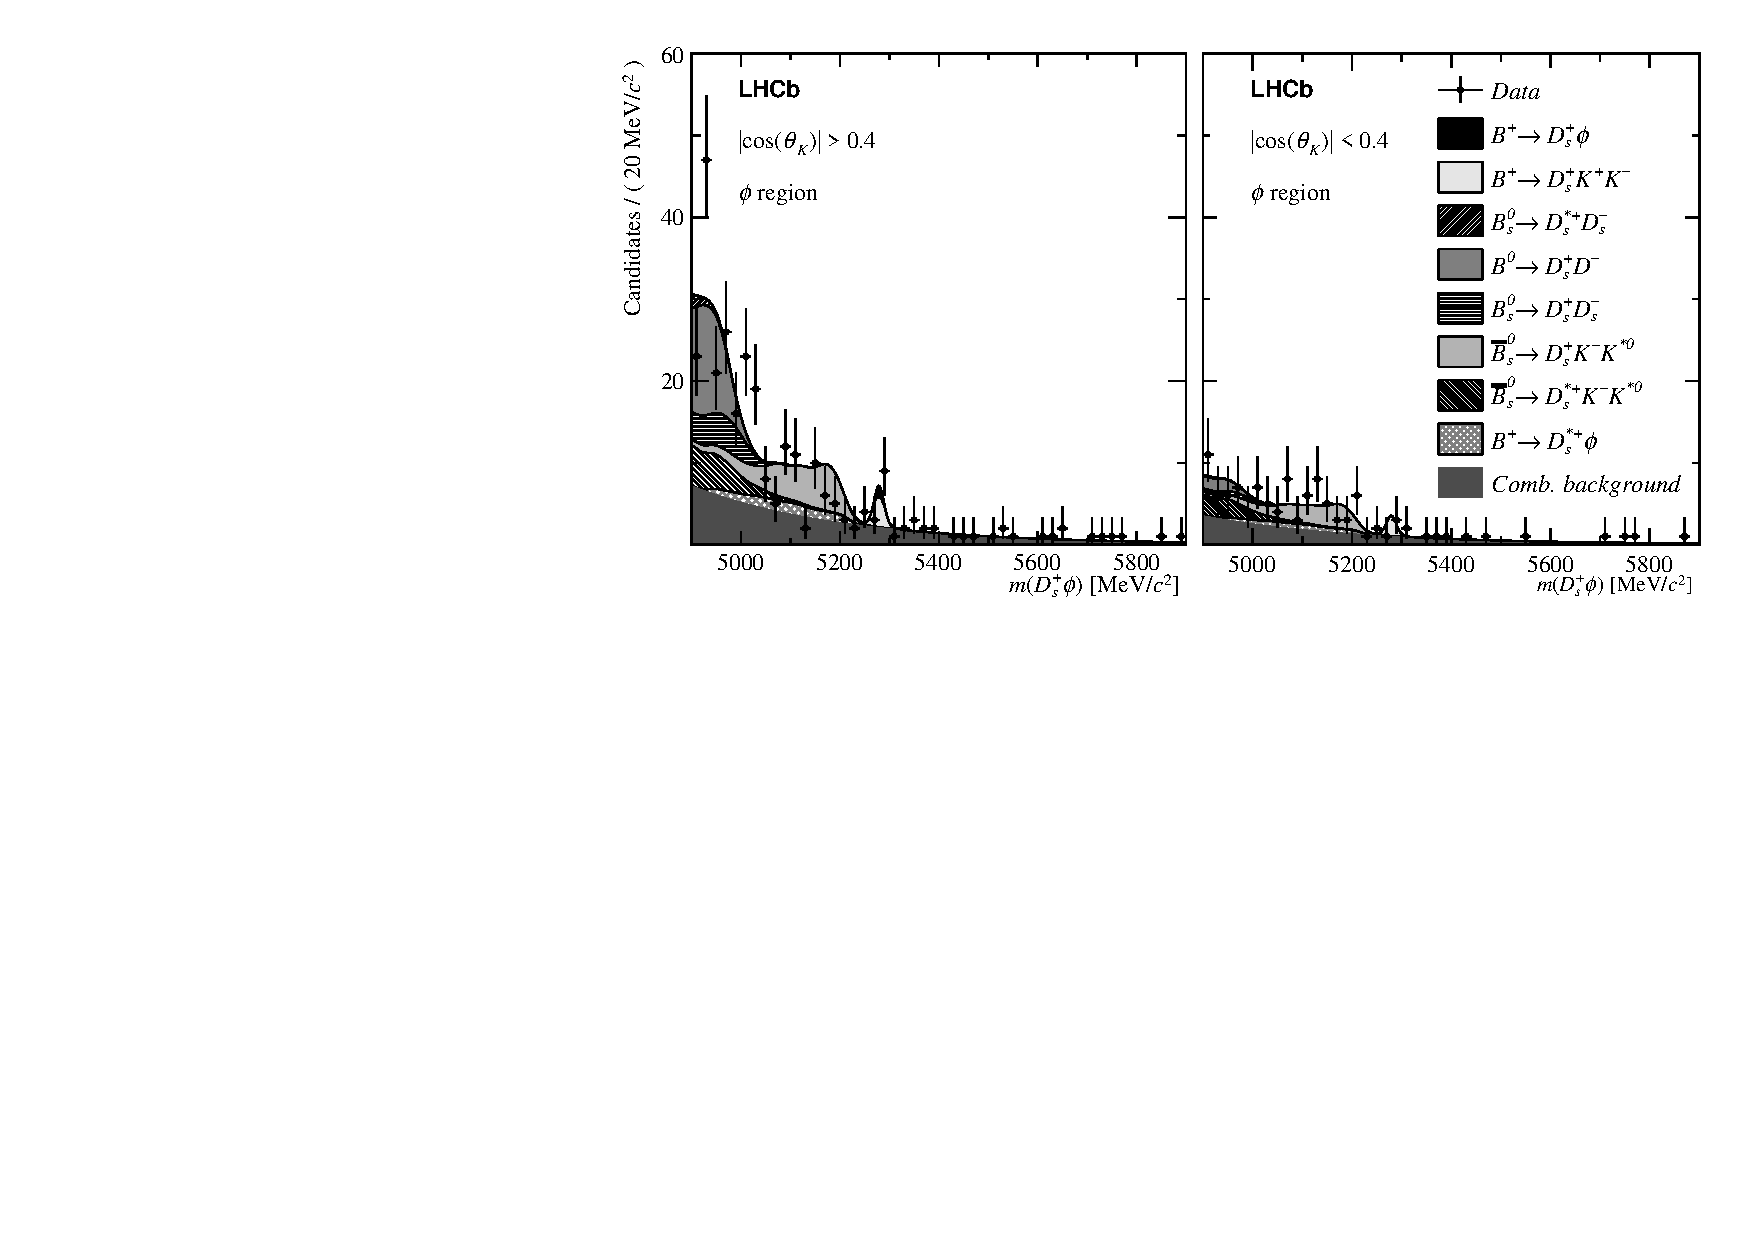
\includegraphics[width=0.7\textwidth]{figs/Appendix_FitCategories/canvas_DsPhi_Ds2KKPi_both_summed_splitHel_splitKKPi_s21_s21r1_s24_s26.pdf}\\
        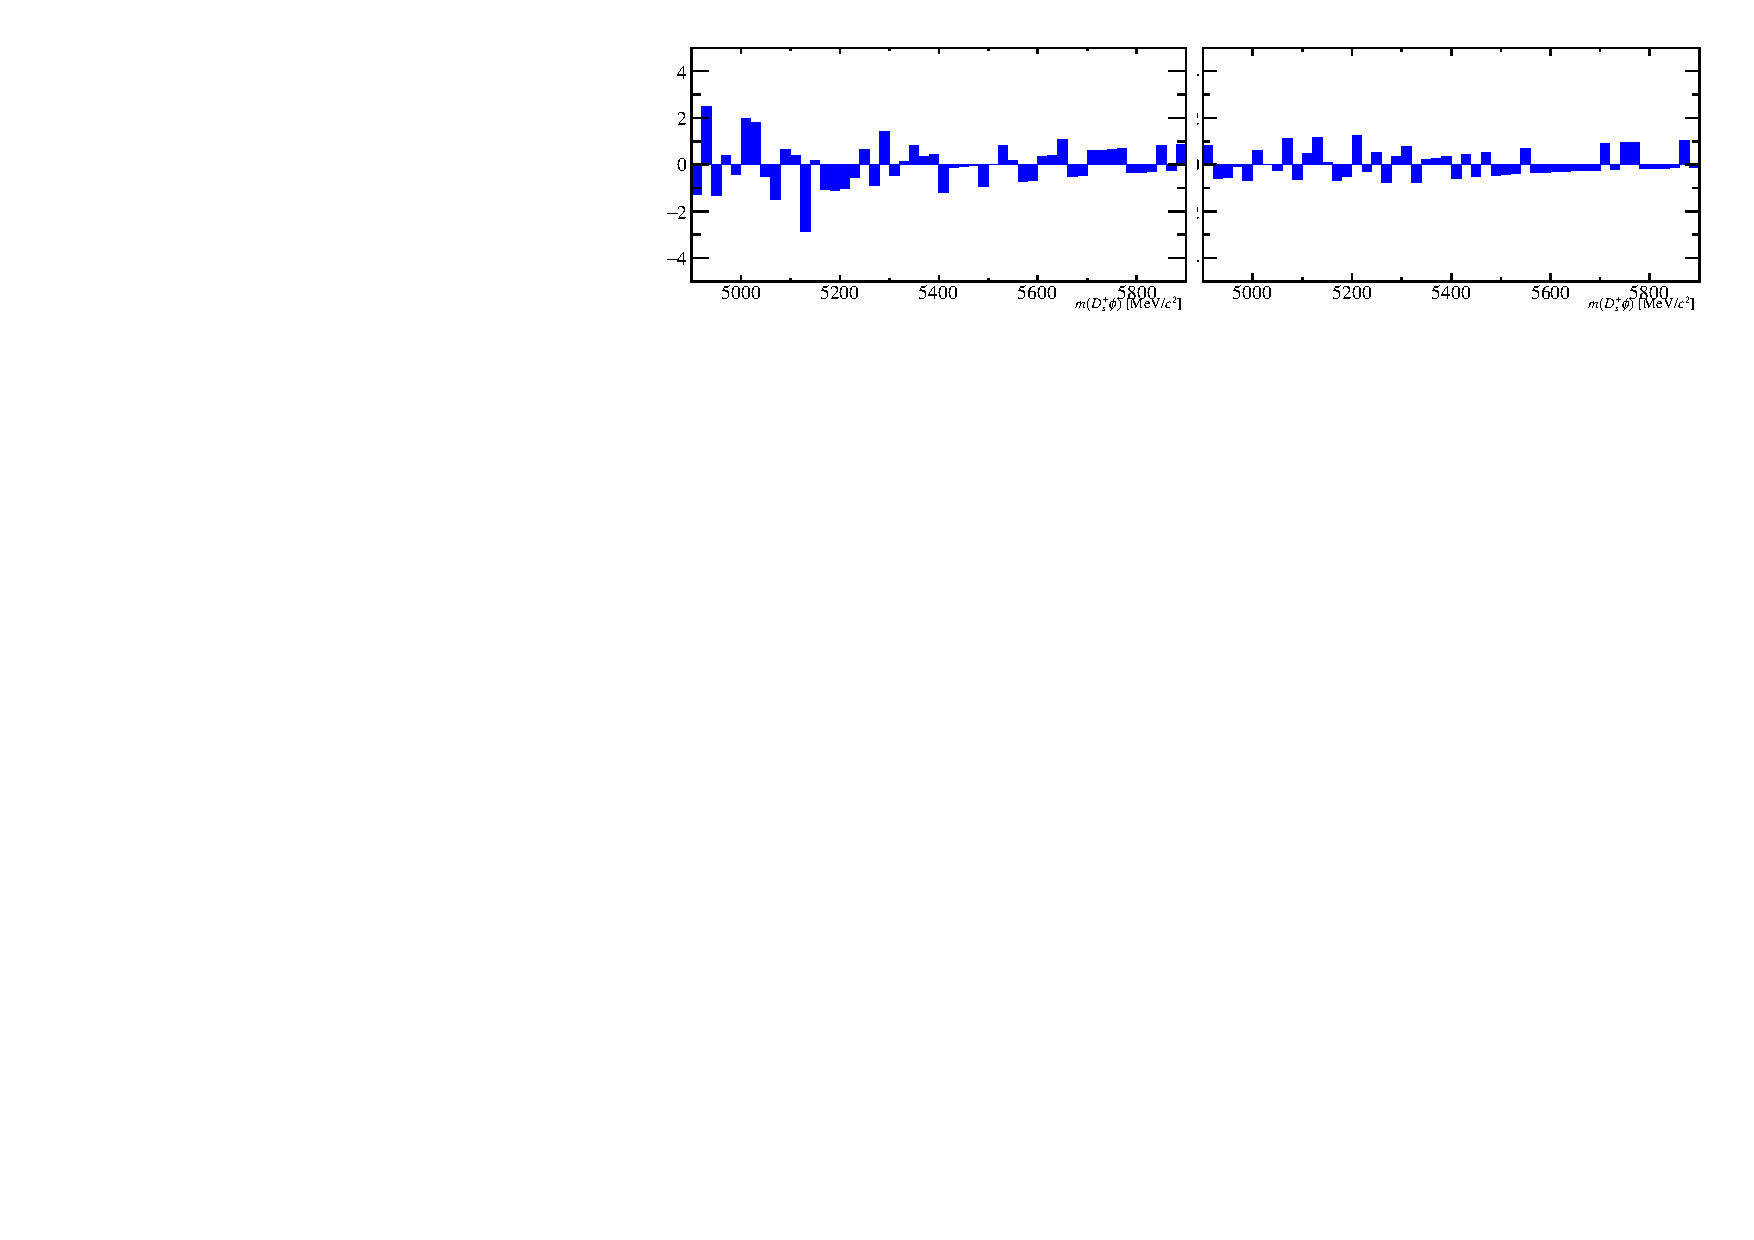
\includegraphics[width=0.7\textwidth]{figs/Appendix_FitCategories/residuals_DsPhi_Ds2KKPi_both_summed_splitHel_splitKKPi_s21_s21r1_s24_s26.pdf}
    \end{subfigure}
    \begin{subfigure}[t]{1.0\textwidth}
        \centering
        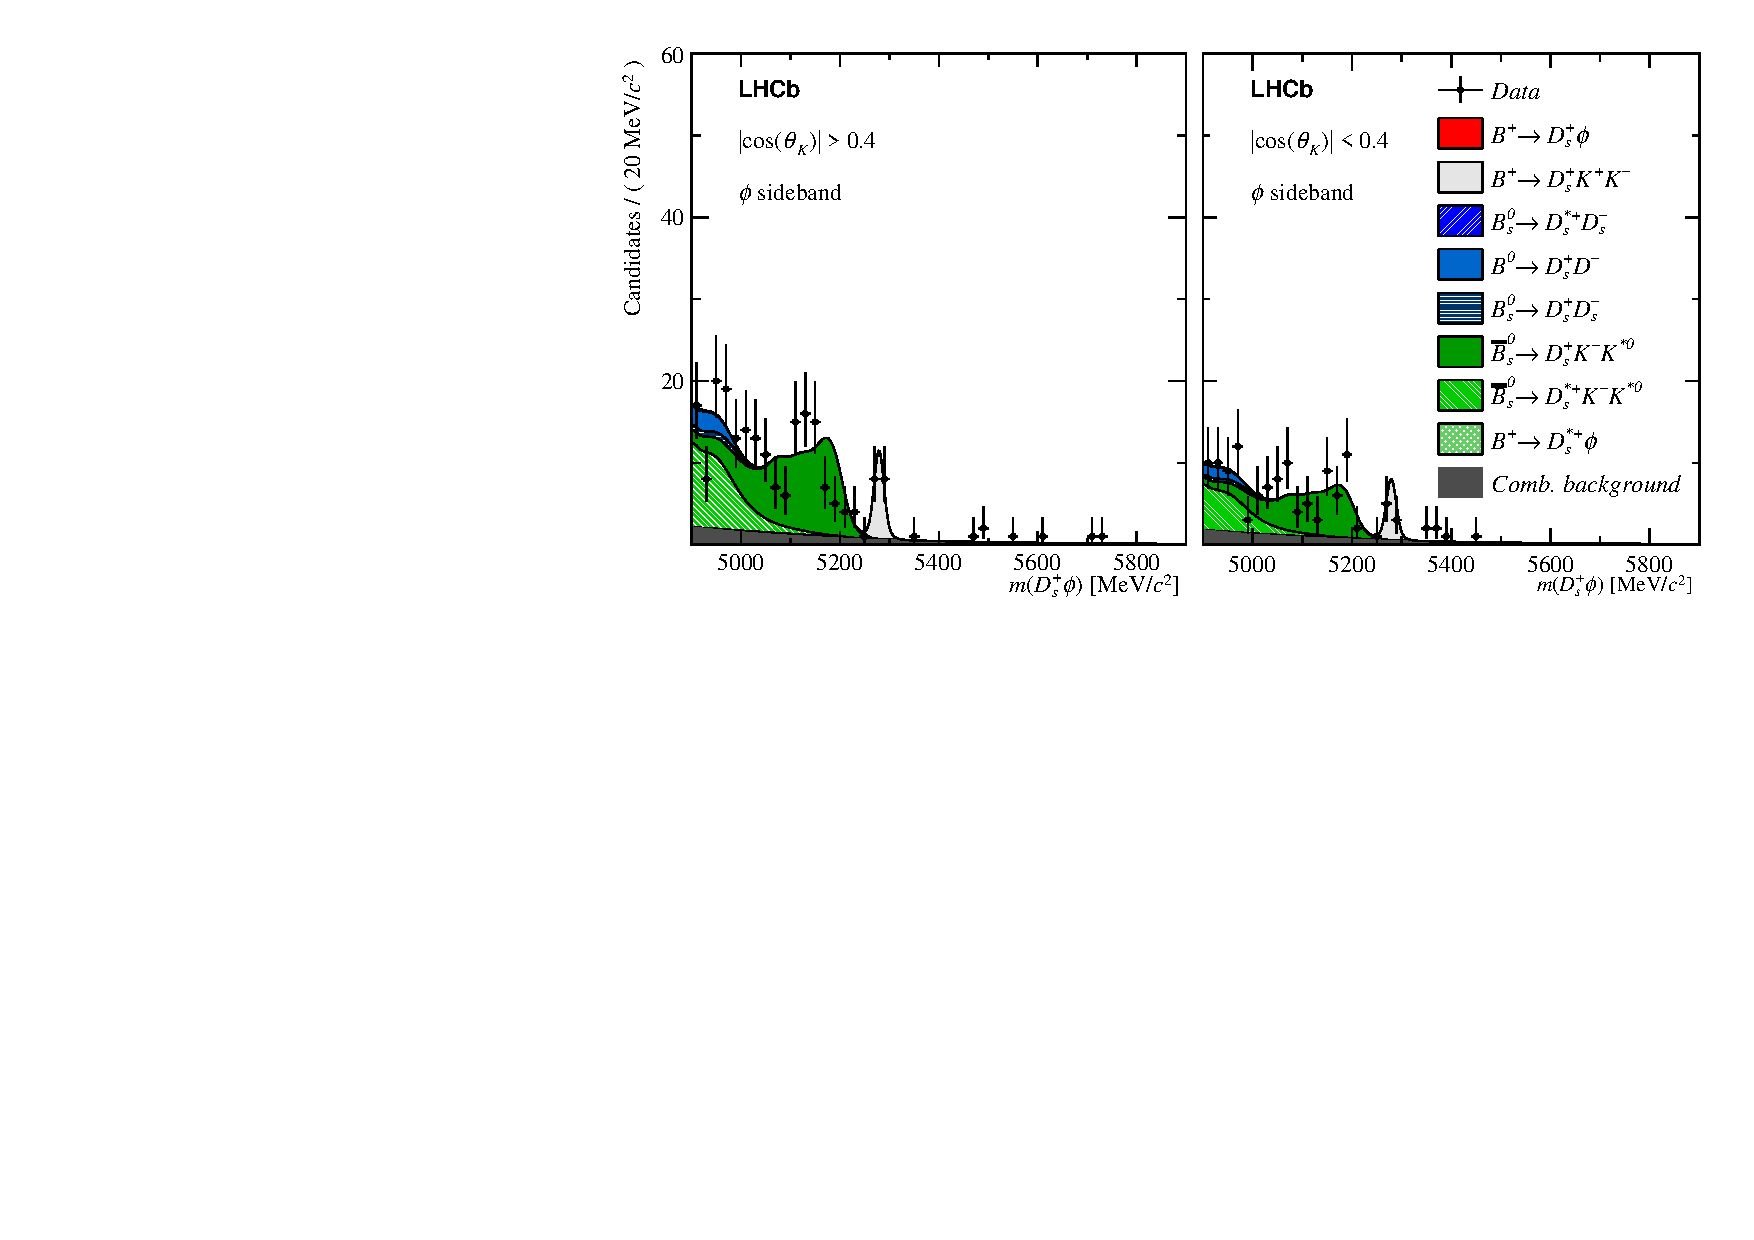
\includegraphics[width=0.7\textwidth]{figs/Appendix_FitCategories/canvas_DsPhiSide_Ds2KKPi_both_summed_splitHel_splitKKPi_s21_s21r1_s24_s26.pdf}\\
        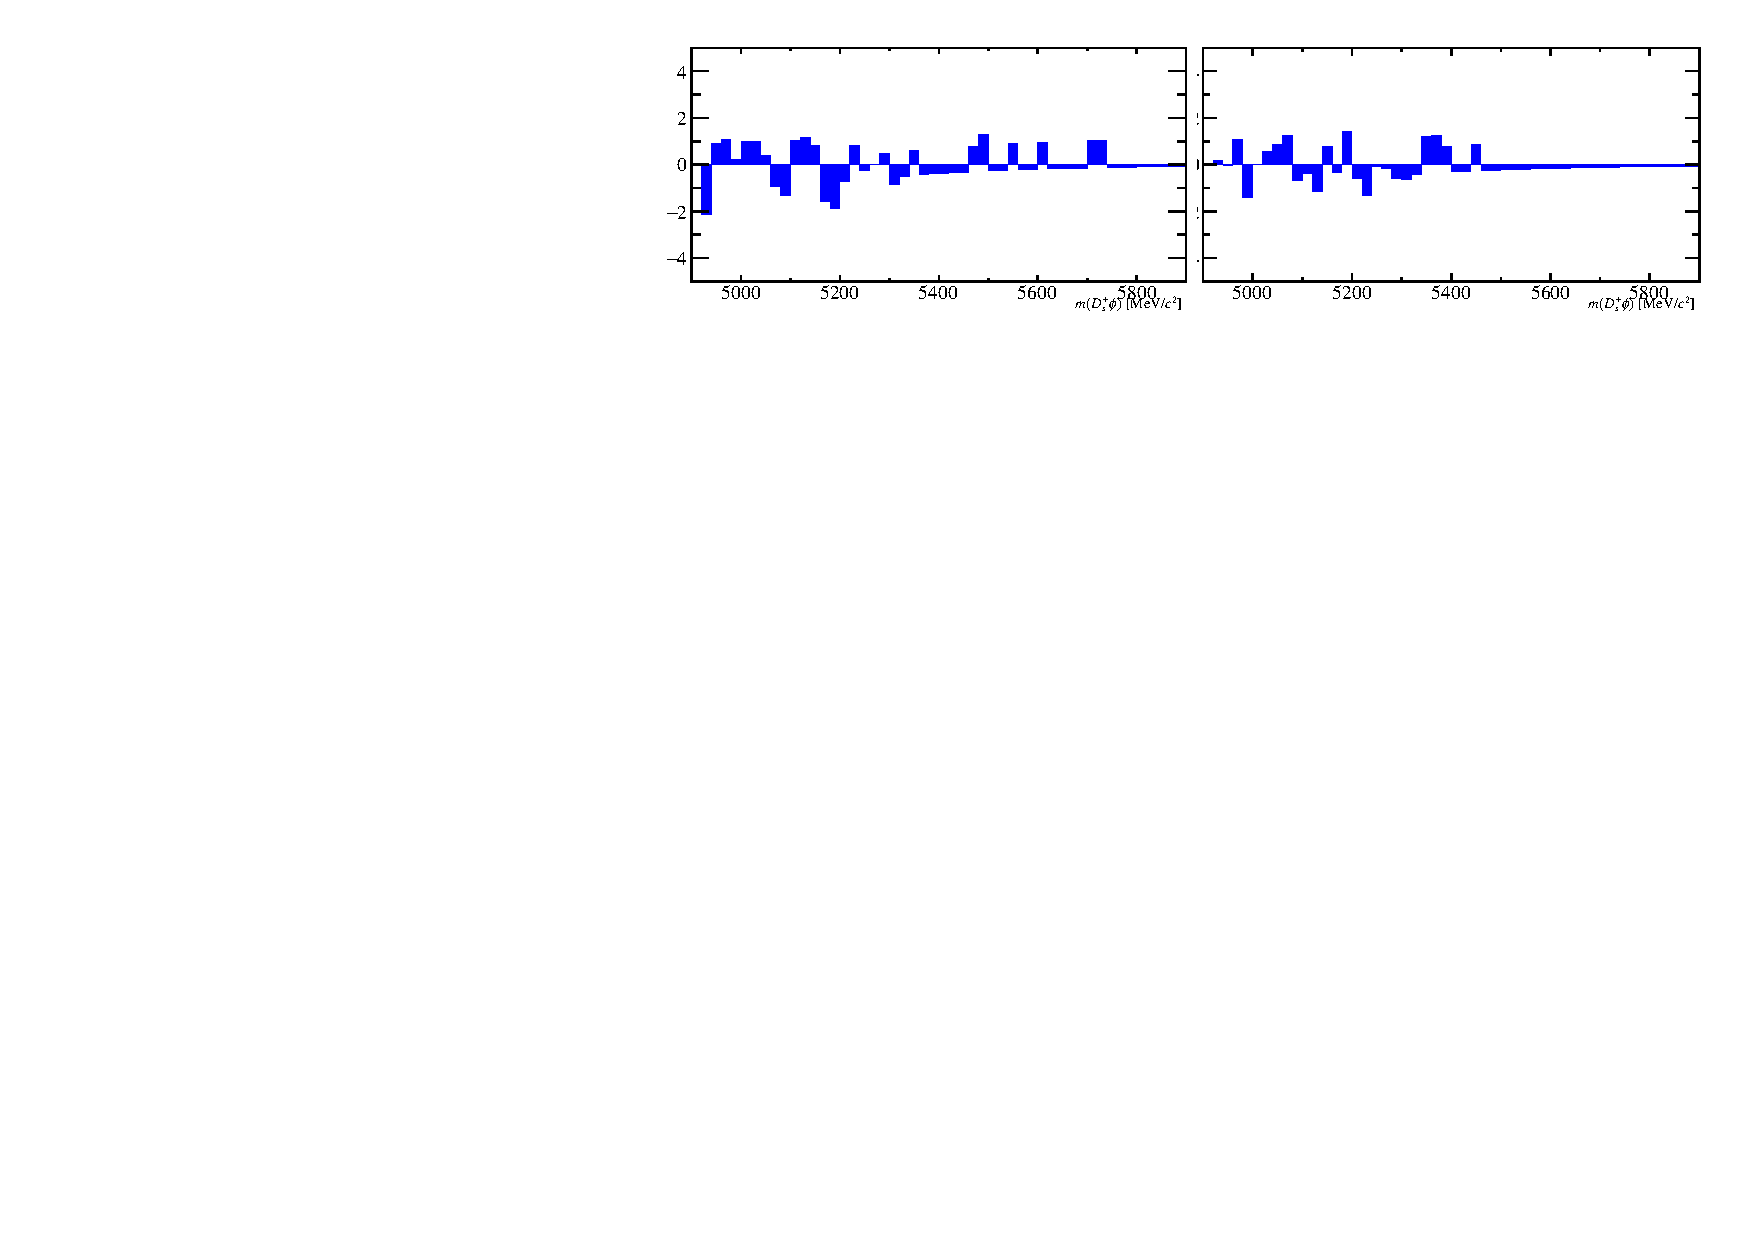
\includegraphics[width=0.7\textwidth]{figs/Appendix_FitCategories/residuals_DsPhiSide_Ds2KKPi_both_summed_splitHel_splitKKPi_s21_s21r1_s24_s26.pdf}
    \end{subfigure}
    \caption{Invariant mass fits to \decay{\Bp}{\Dsp\phiz} candidates with \decay{\Dsp}{\Kp\Km\pip} (excluding \decay{\Dsp}{\phiz\pip}).}
\end{figure}
%%%%%%%%%%%%%%%%%%%%%%%%%%%%%%%%%%%%%%%%%%%%%%%%%%%%%%%%%%
%%%%%%%%%%%%%%%%%%%%%%%%%%%%%%%%%%%%%%%%%%%%%%%%%%%%%%%%%%
\begin{figure}[!h]
    \centering
    \begin{subfigure}[t]{1.0\textwidth}
        \centering
        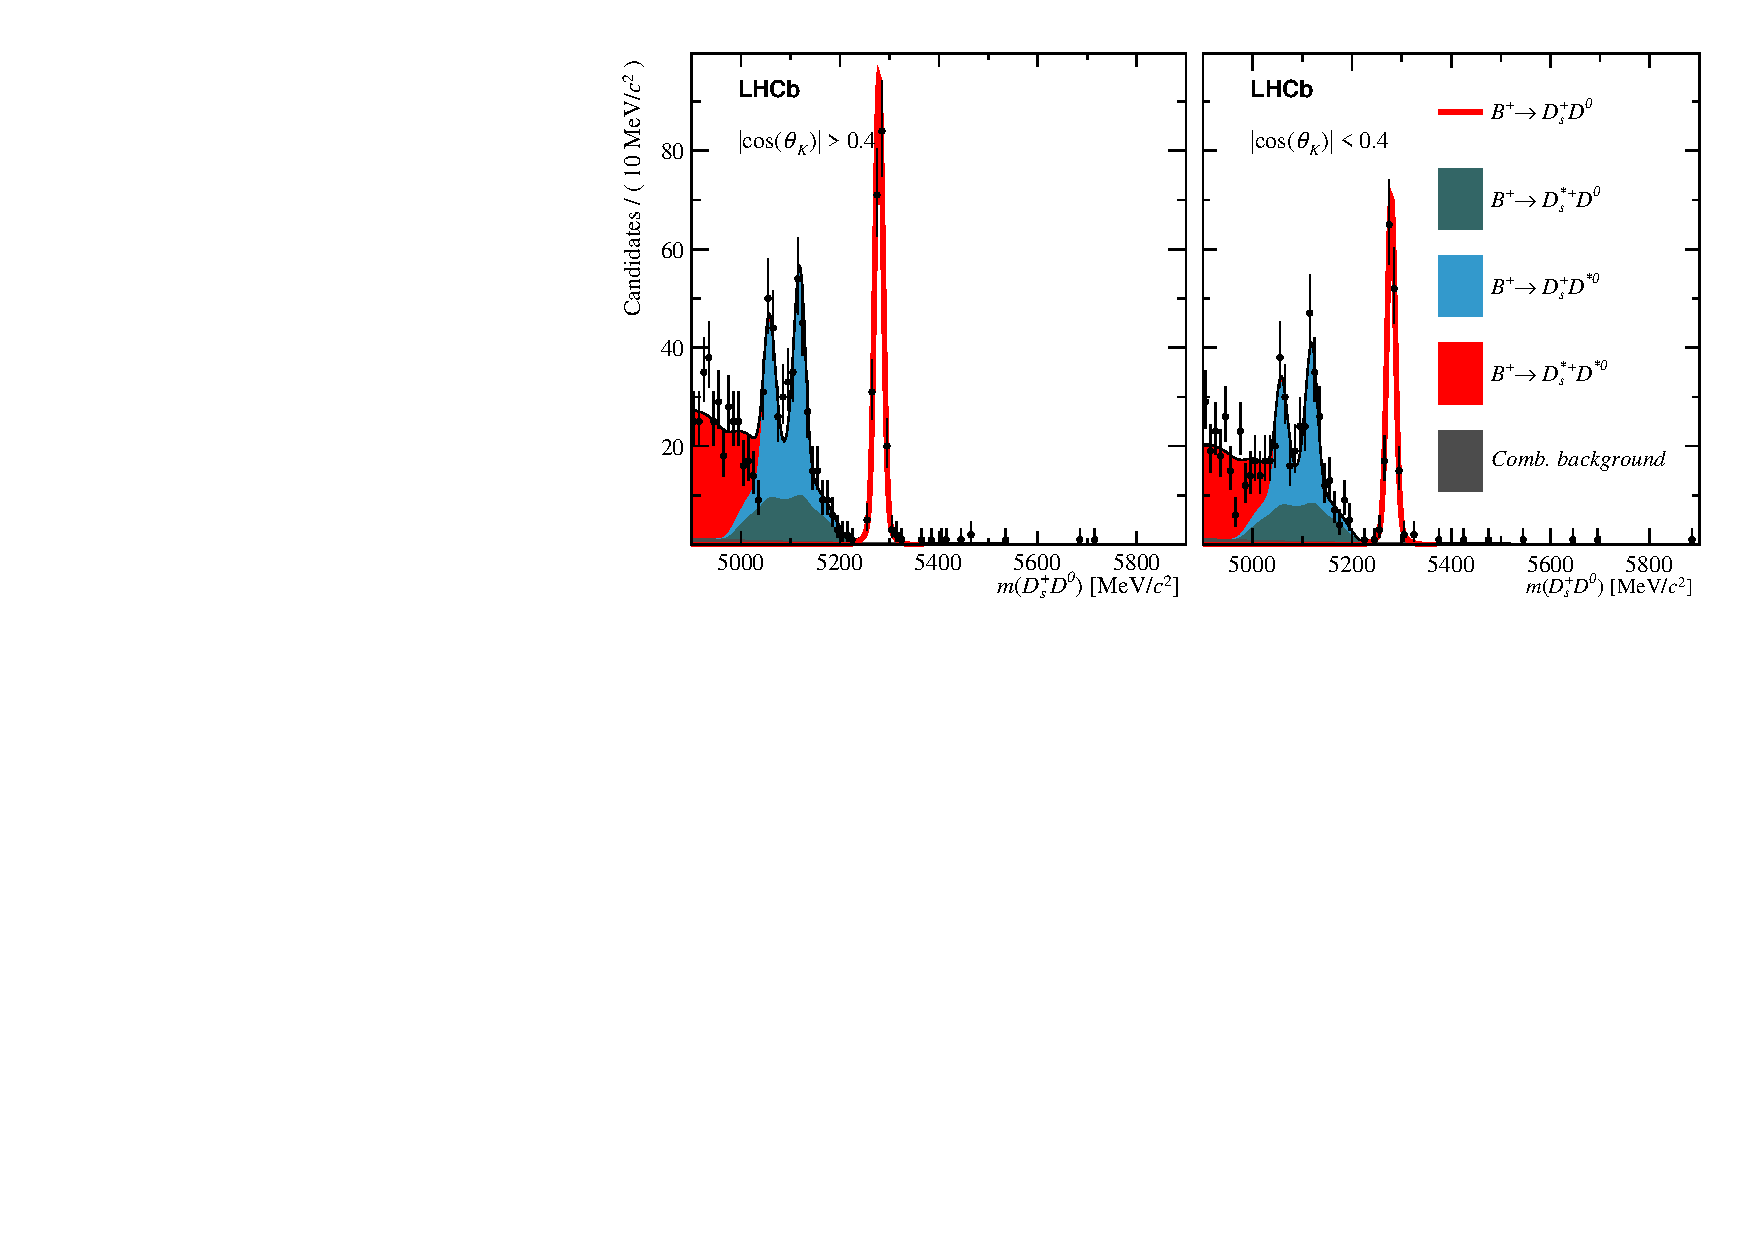
\includegraphics[width=0.7\textwidth]{figs/Appendix_FitCategories/canvas_DsD0_Ds2PiPiPi_both_summed_splitHel_splitKKPi_s21_s21r1_s24_s26.pdf}\\
        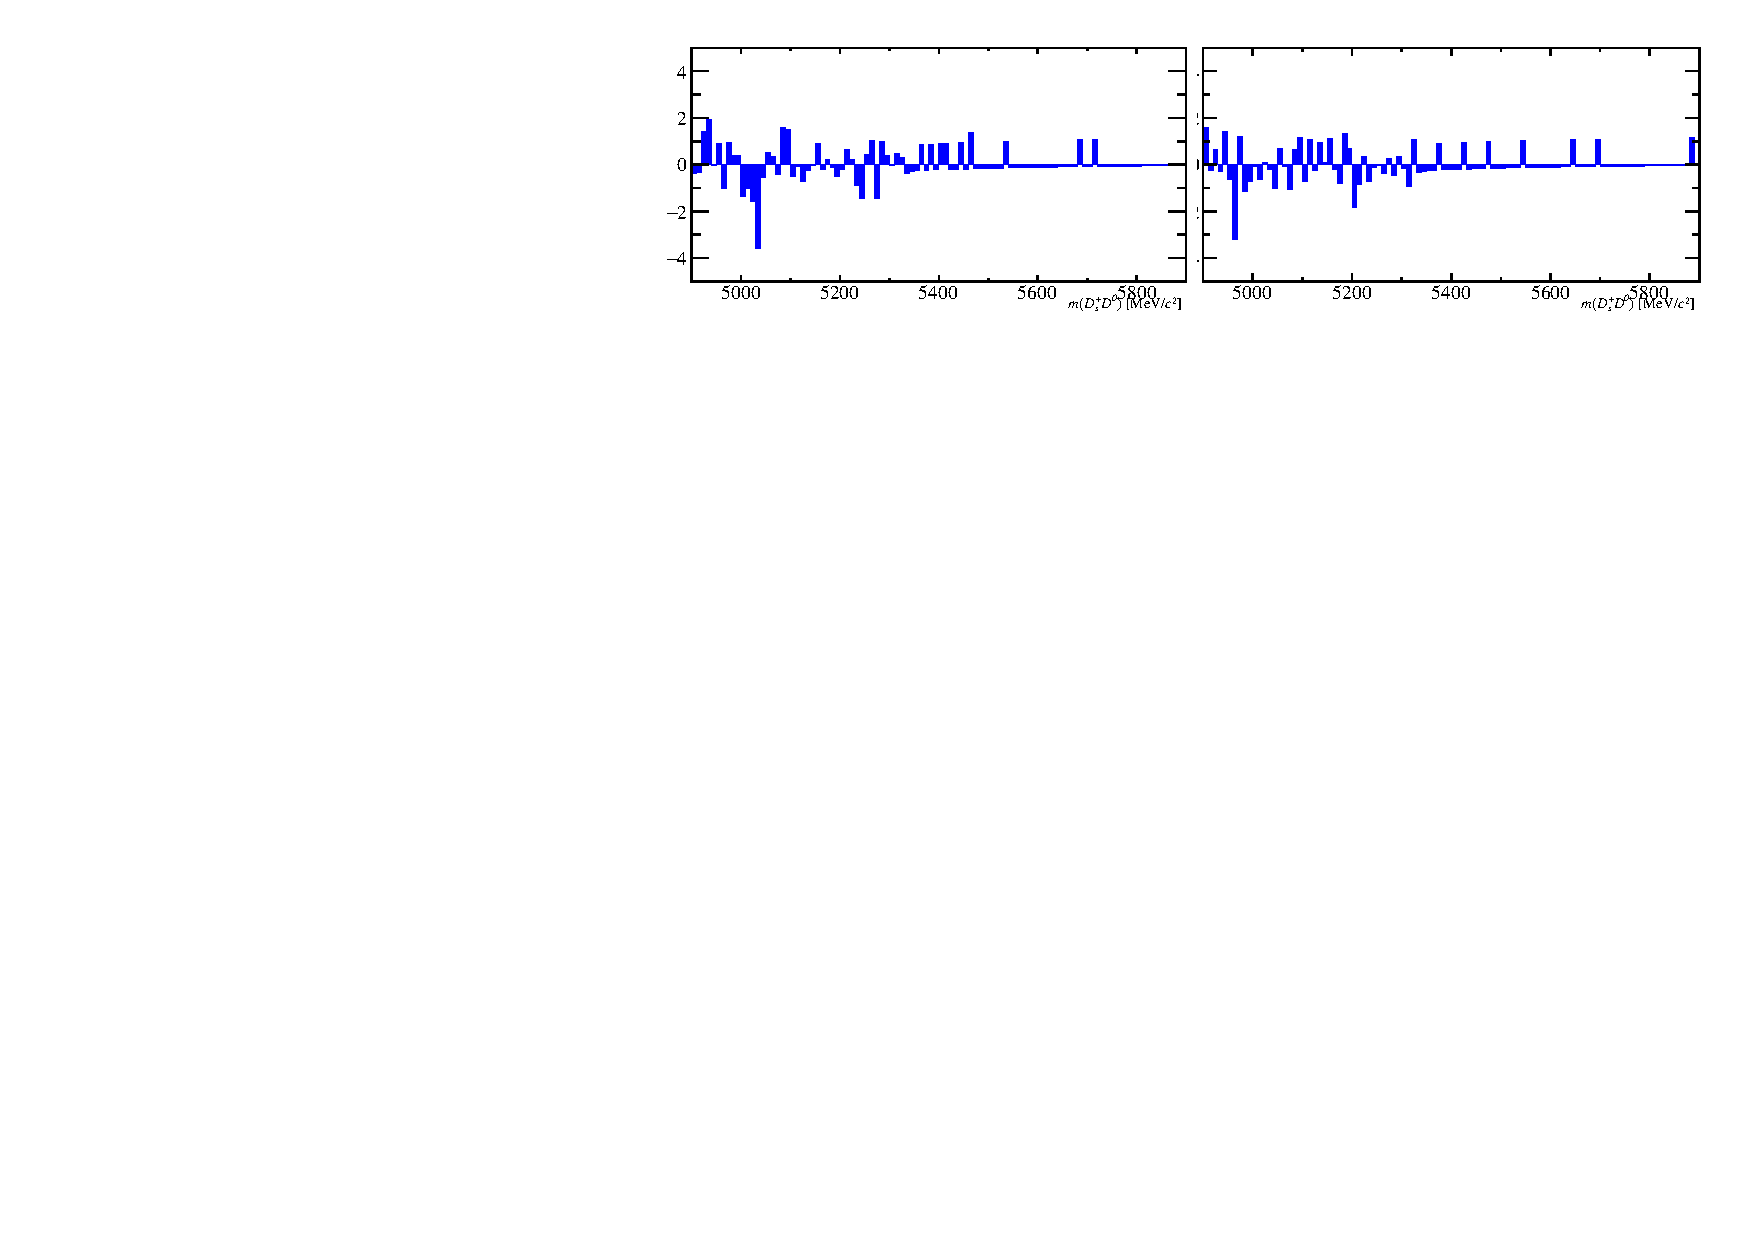
\includegraphics[width=0.7\textwidth]{figs/Appendix_FitCategories/residuals_DsD0_Ds2PiPiPi_both_summed_splitHel_splitKKPi_s21_s21r1_s24_s26.pdf}
    \end{subfigure}
    \begin{subfigure}[t]{1.0\textwidth}
        \centering
        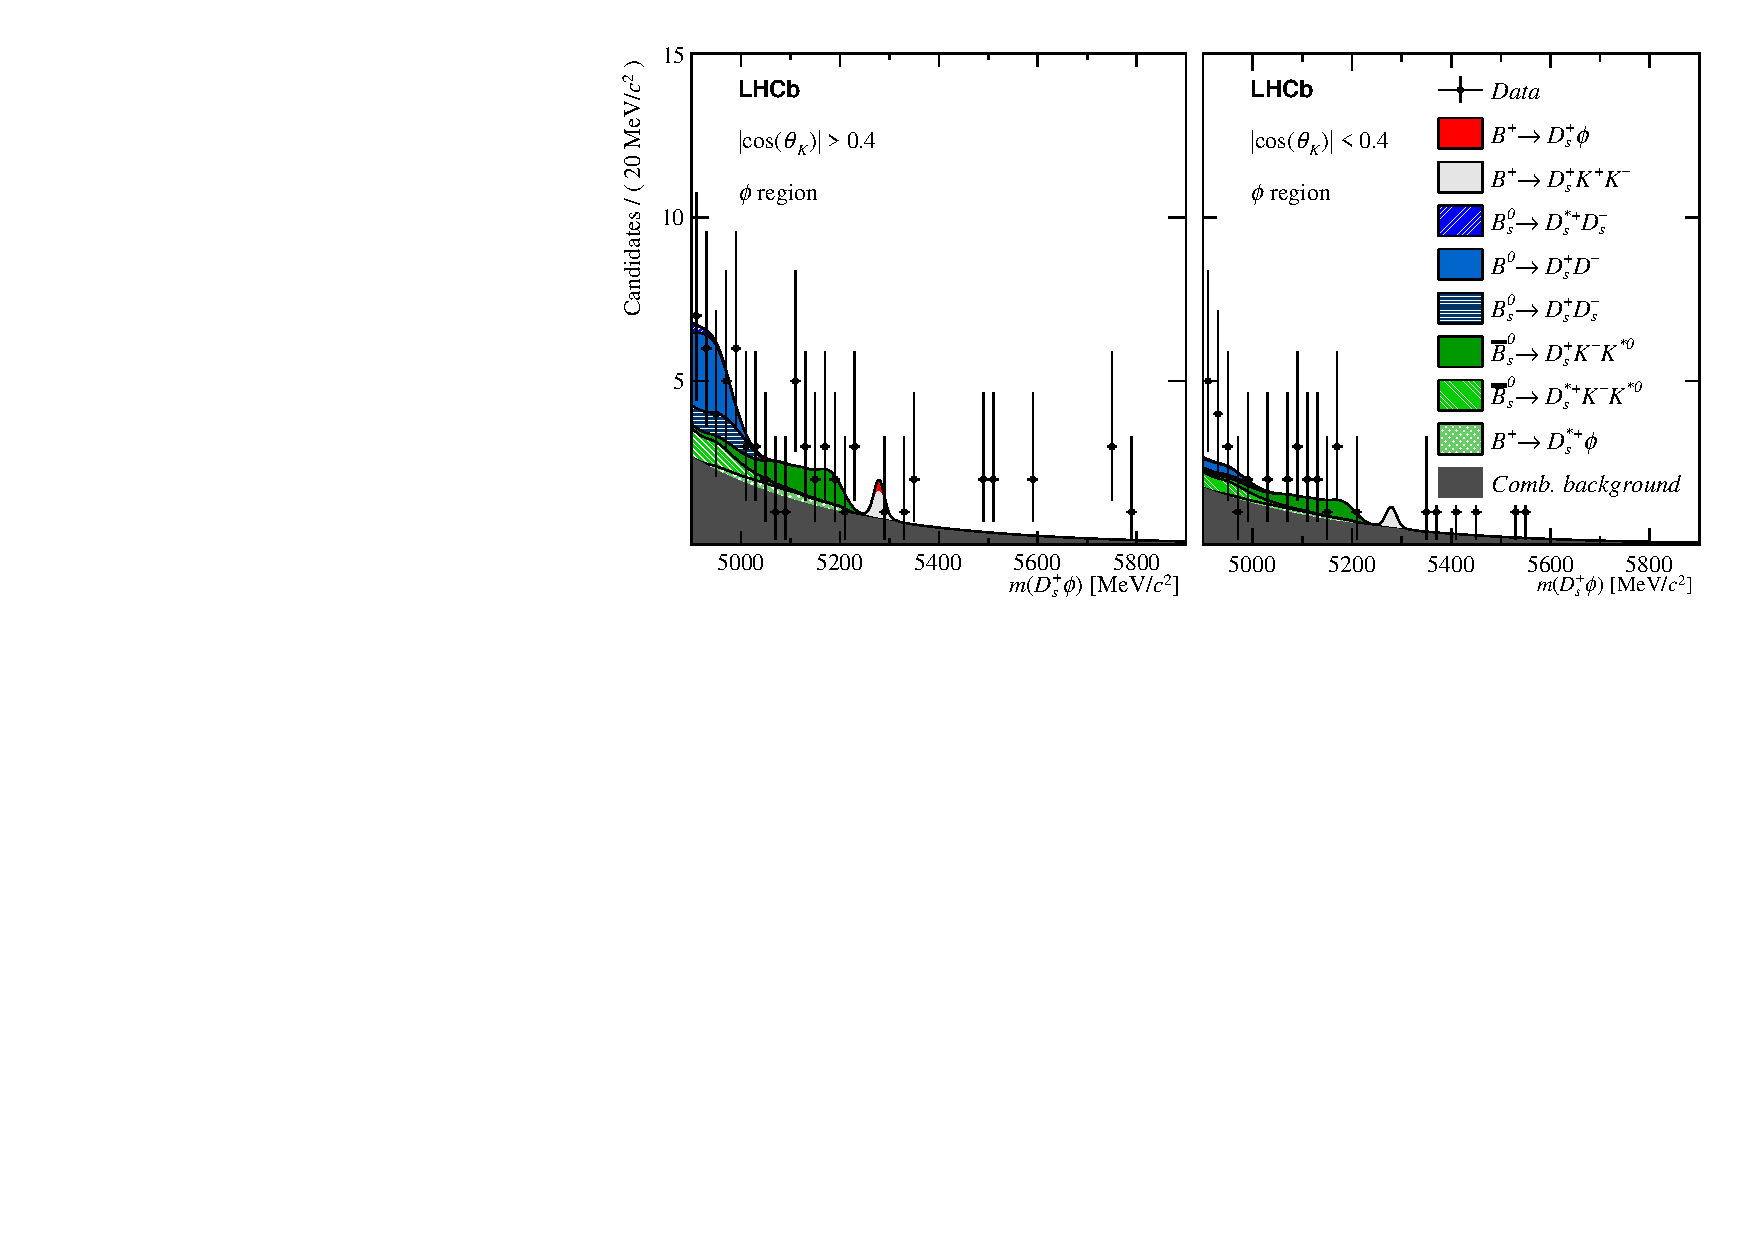
\includegraphics[width=0.7\textwidth]{figs/Appendix_FitCategories/canvas_DsPhi_Ds2PiPiPi_both_summed_splitHel_splitKKPi_s21_s21r1_s24_s26.pdf}\\
        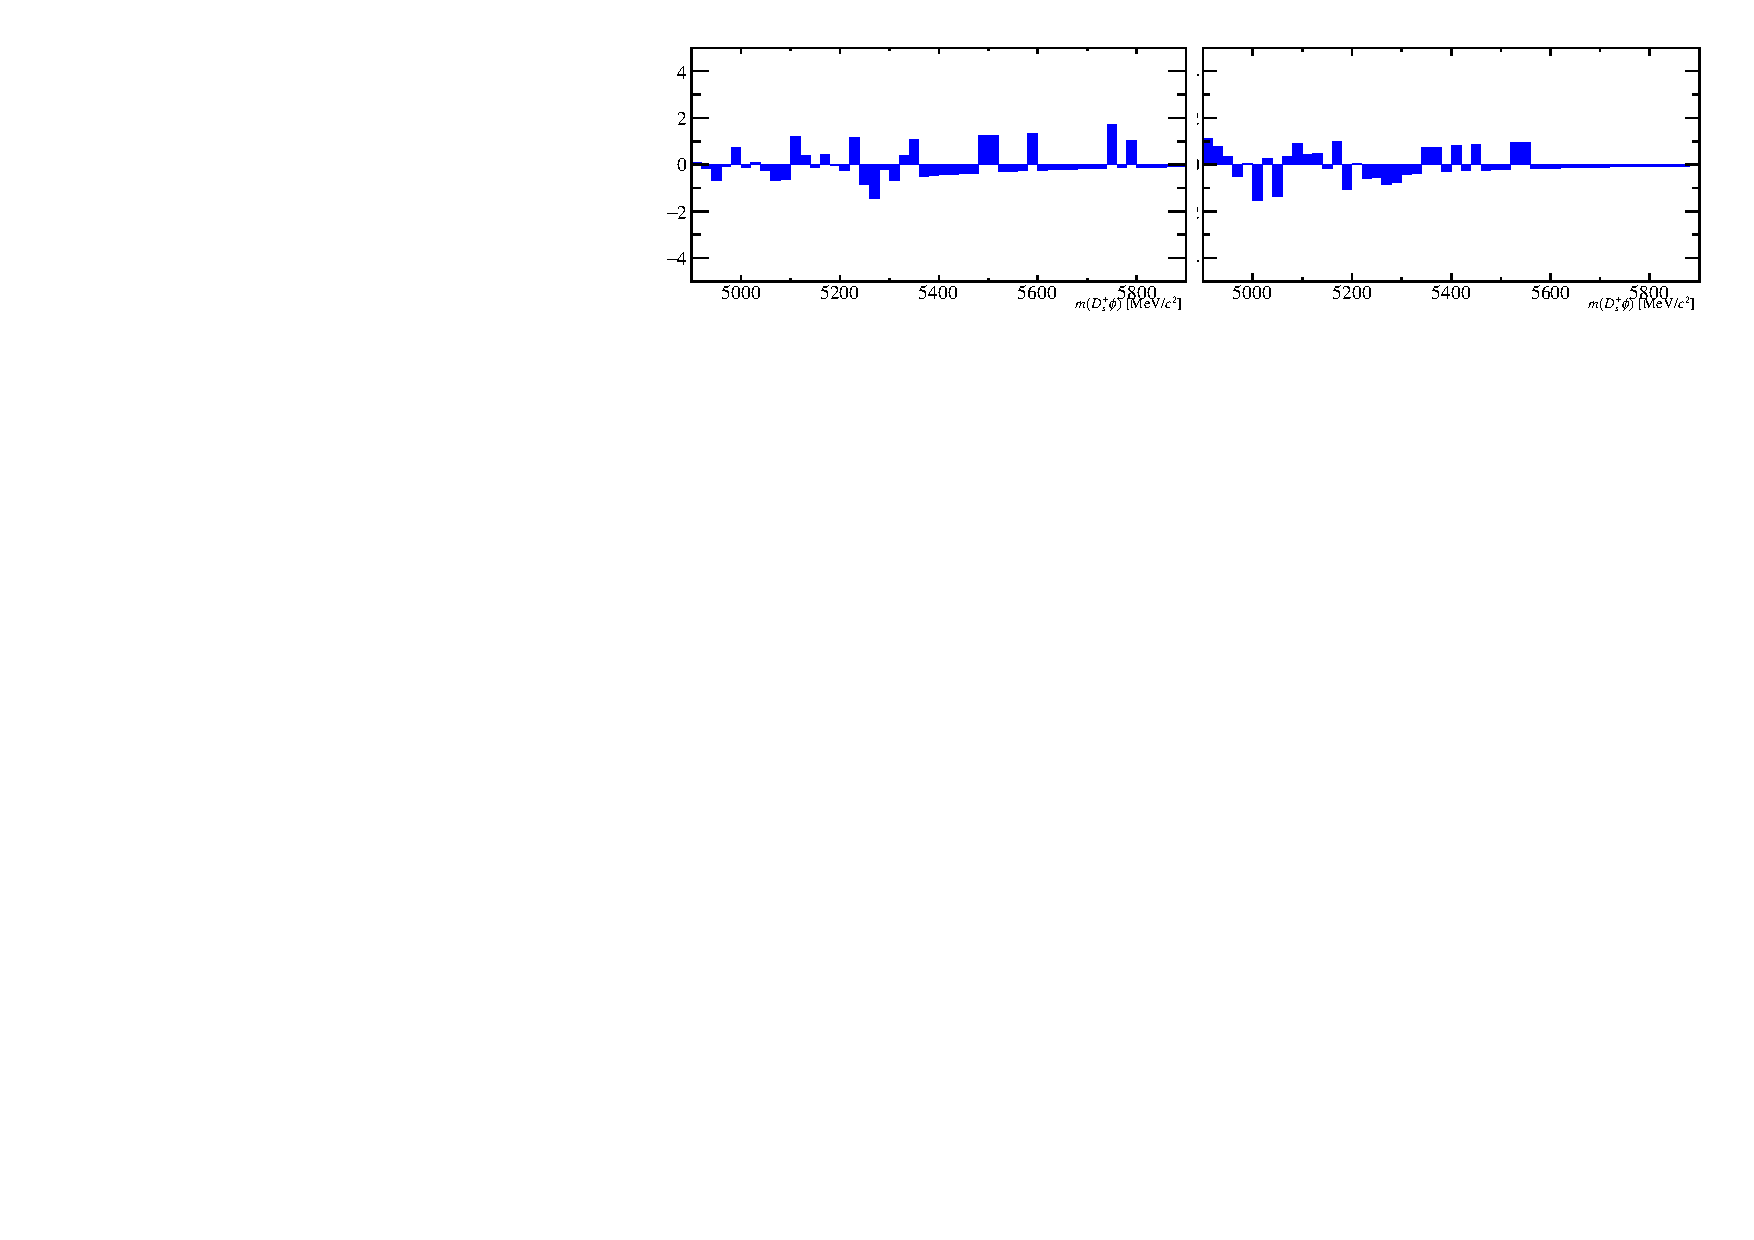
\includegraphics[width=0.7\textwidth]{figs/Appendix_FitCategories/residuals_DsPhi_Ds2PiPiPi_both_summed_splitHel_splitKKPi_s21_s21r1_s24_s26.pdf}
    \end{subfigure}
    \begin{subfigure}[t]{1.0\textwidth}
        \centering
        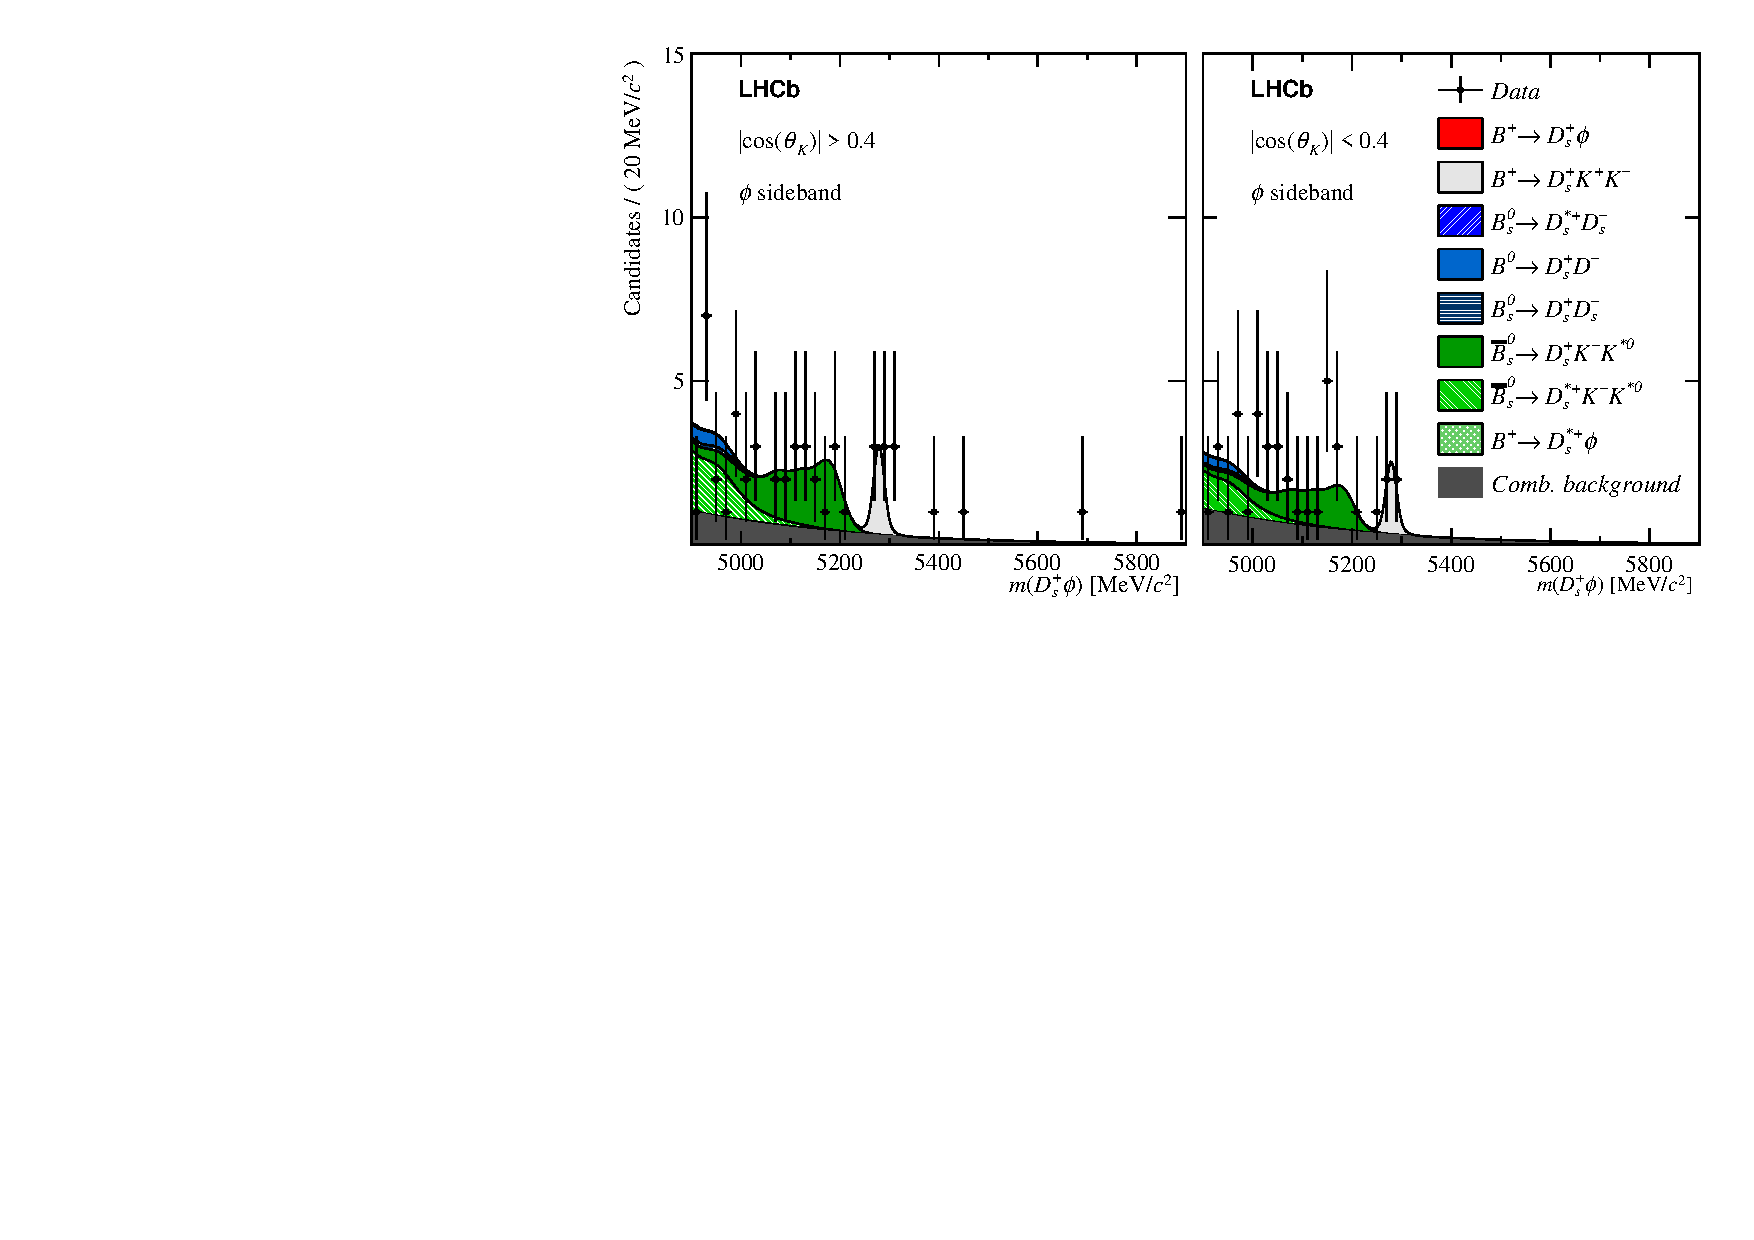
\includegraphics[width=0.7\textwidth]{figs/Appendix_FitCategories/canvas_DsPhiSide_Ds2PiPiPi_both_summed_splitHel_splitKKPi_s21_s21r1_s24_s26.pdf}\\
        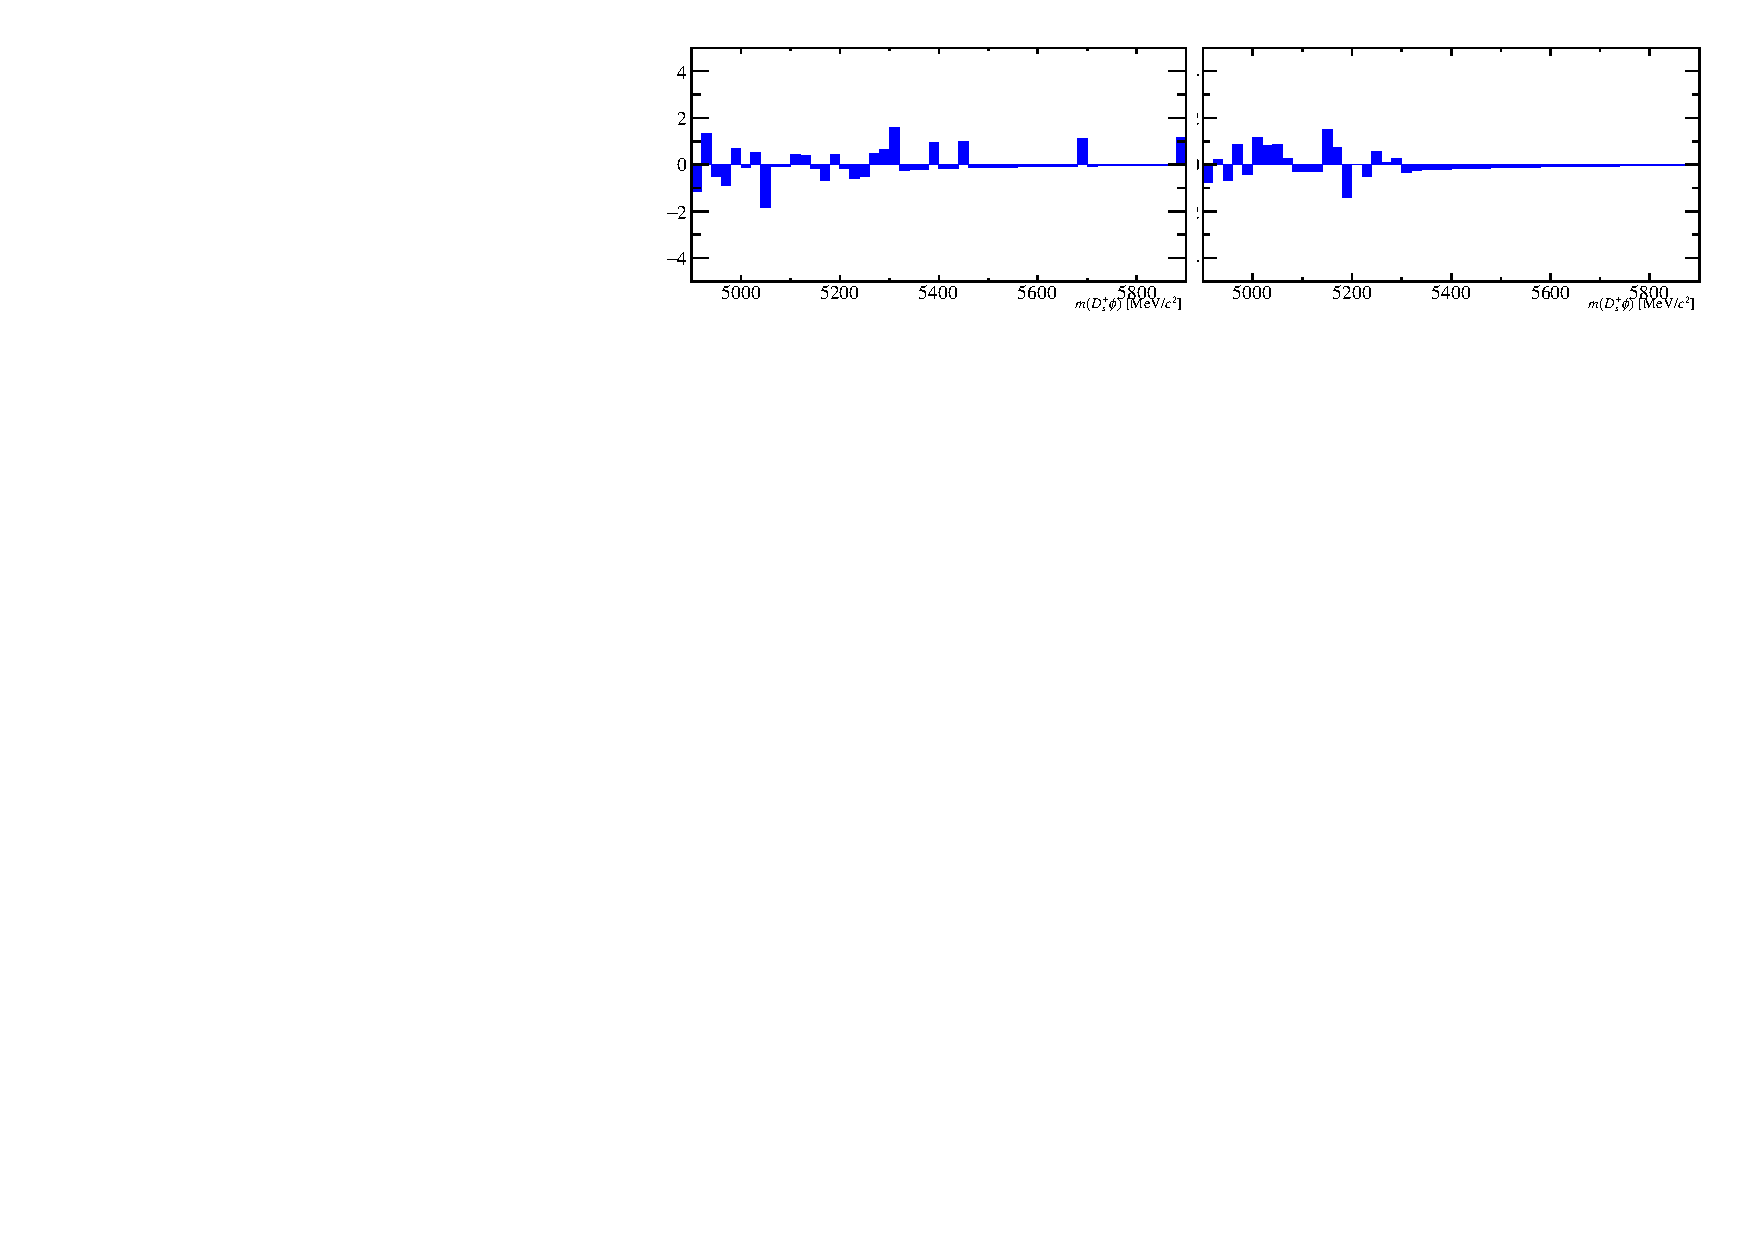
\includegraphics[width=0.7\textwidth]{figs/Appendix_FitCategories/residuals_DsPhiSide_Ds2PiPiPi_both_summed_splitHel_splitKKPi_s21_s21r1_s24_s26.pdf}
    \end{subfigure}
    \caption{Invariant mass fits to \decay{\Bp}{\Dsp\phiz} candidates with \decay{\Dsp}{\pip\pim\pip}.}
\end{figure}
%%%%%%%%%%%%%%%%%%%%%%%%%%%%%%%%%%%%%%%%%%%%%%%%%%%%%%%%%%
%%%%%%%%%%%%%%%%%%%%%%%%%%%%%%%%%%%%%%%%%%%%%%%%%%%%%%%%%%
\begin{figure}[!h]
    \centering
    \begin{subfigure}[t]{1.0\textwidth}
        \centering
        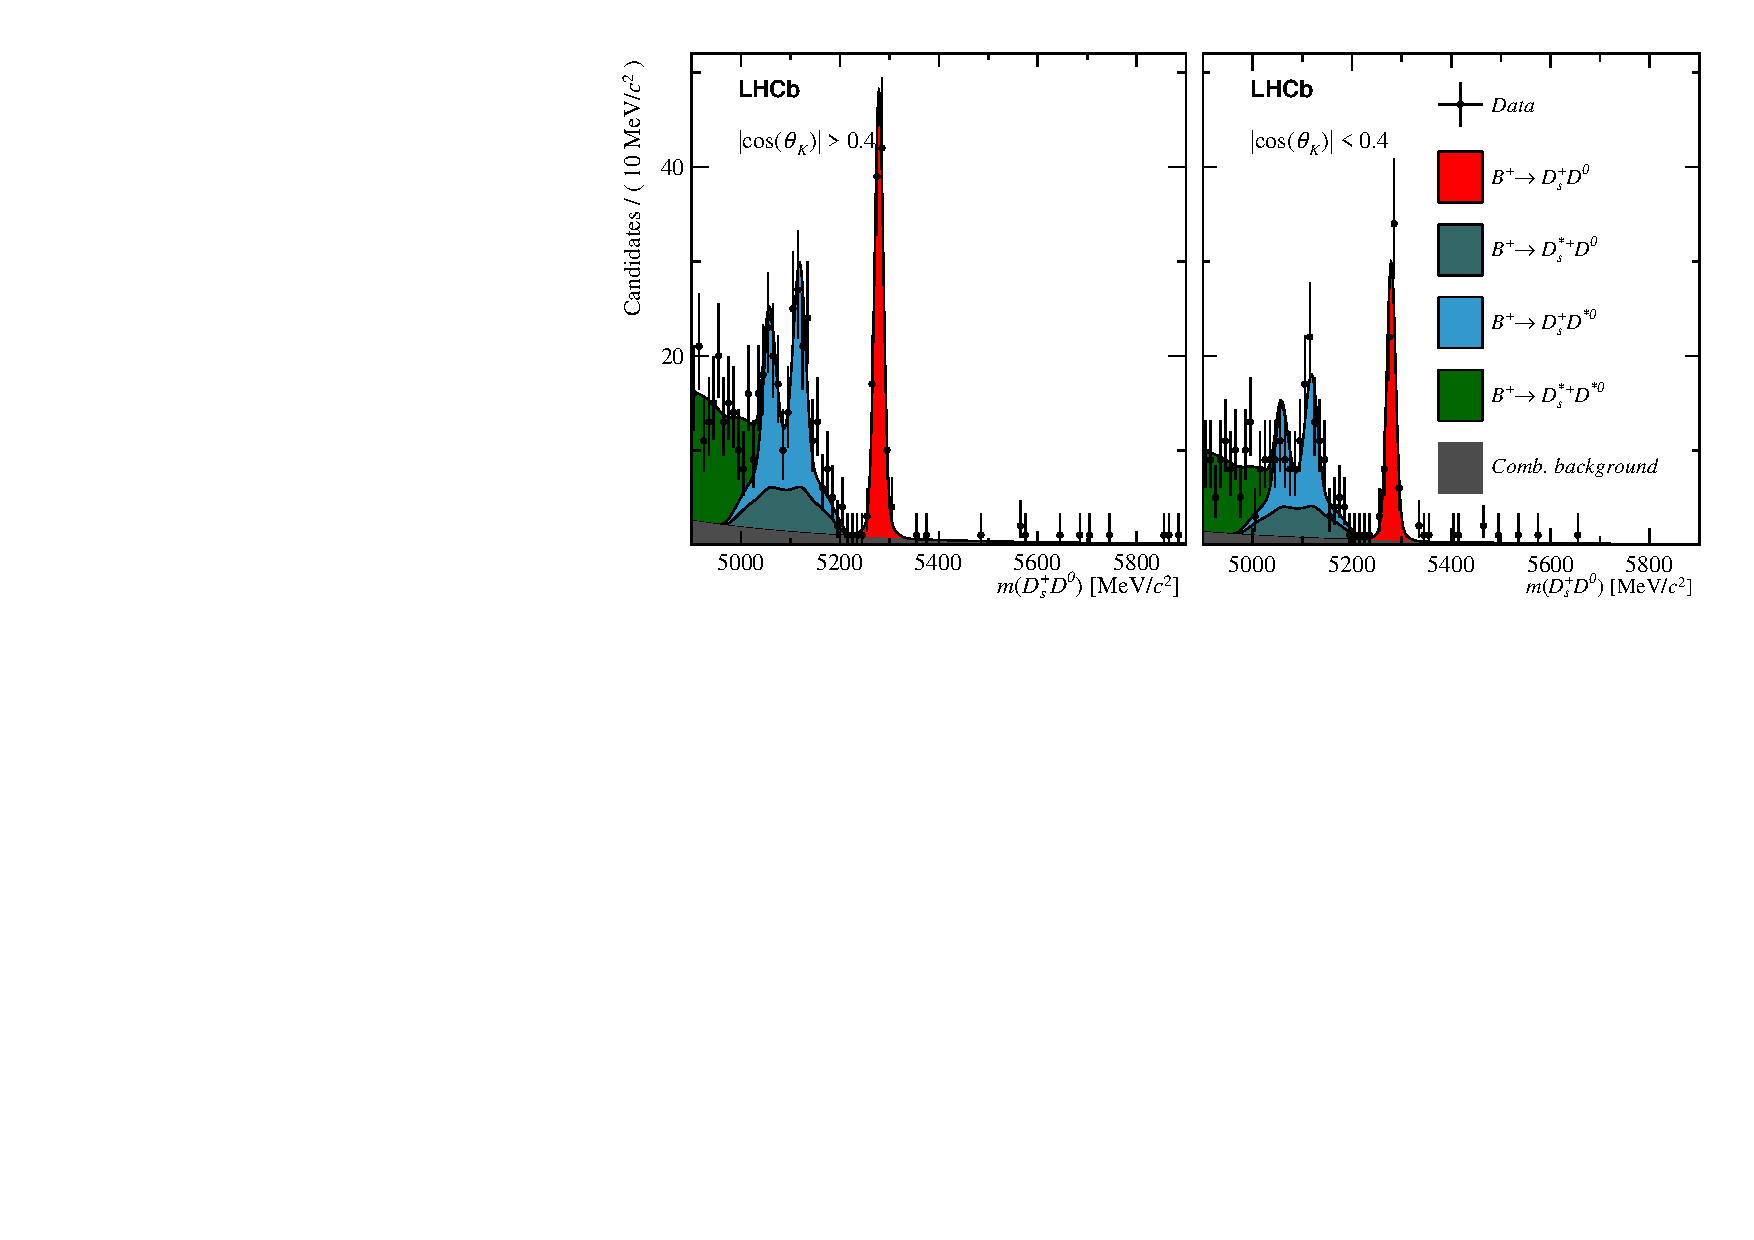
\includegraphics[width=0.7\textwidth]{figs/Appendix_FitCategories/canvas_DsD0_Ds2KPiPi_both_summed_splitHel_splitKKPi_s21_s21r1_s24_s26.pdf}\\
        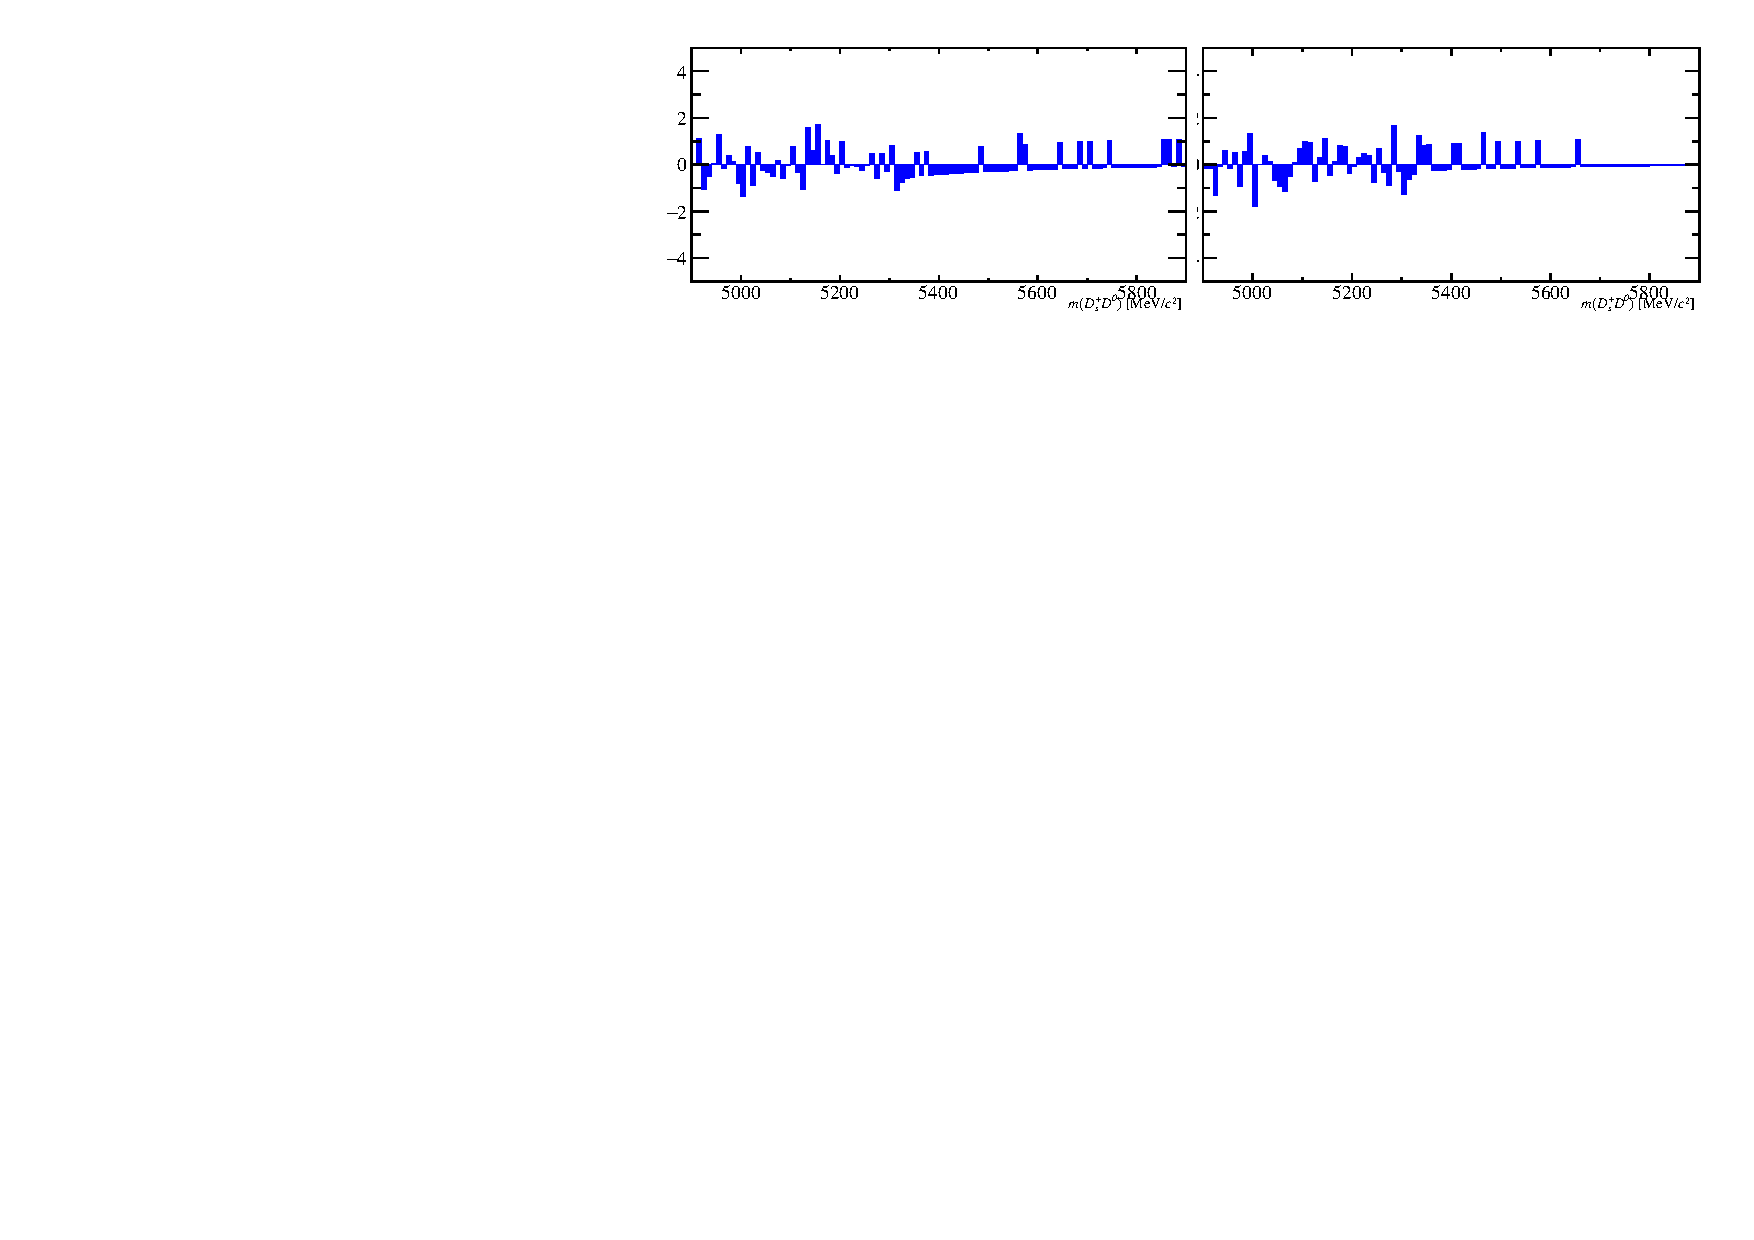
\includegraphics[width=0.7\textwidth]{figs/Appendix_FitCategories/residuals_DsD0_Ds2KPiPi_both_summed_splitHel_splitKKPi_s21_s21r1_s24_s26.pdf}
    \end{subfigure}
    \begin{subfigure}[t]{1.0\textwidth}
        \centering
        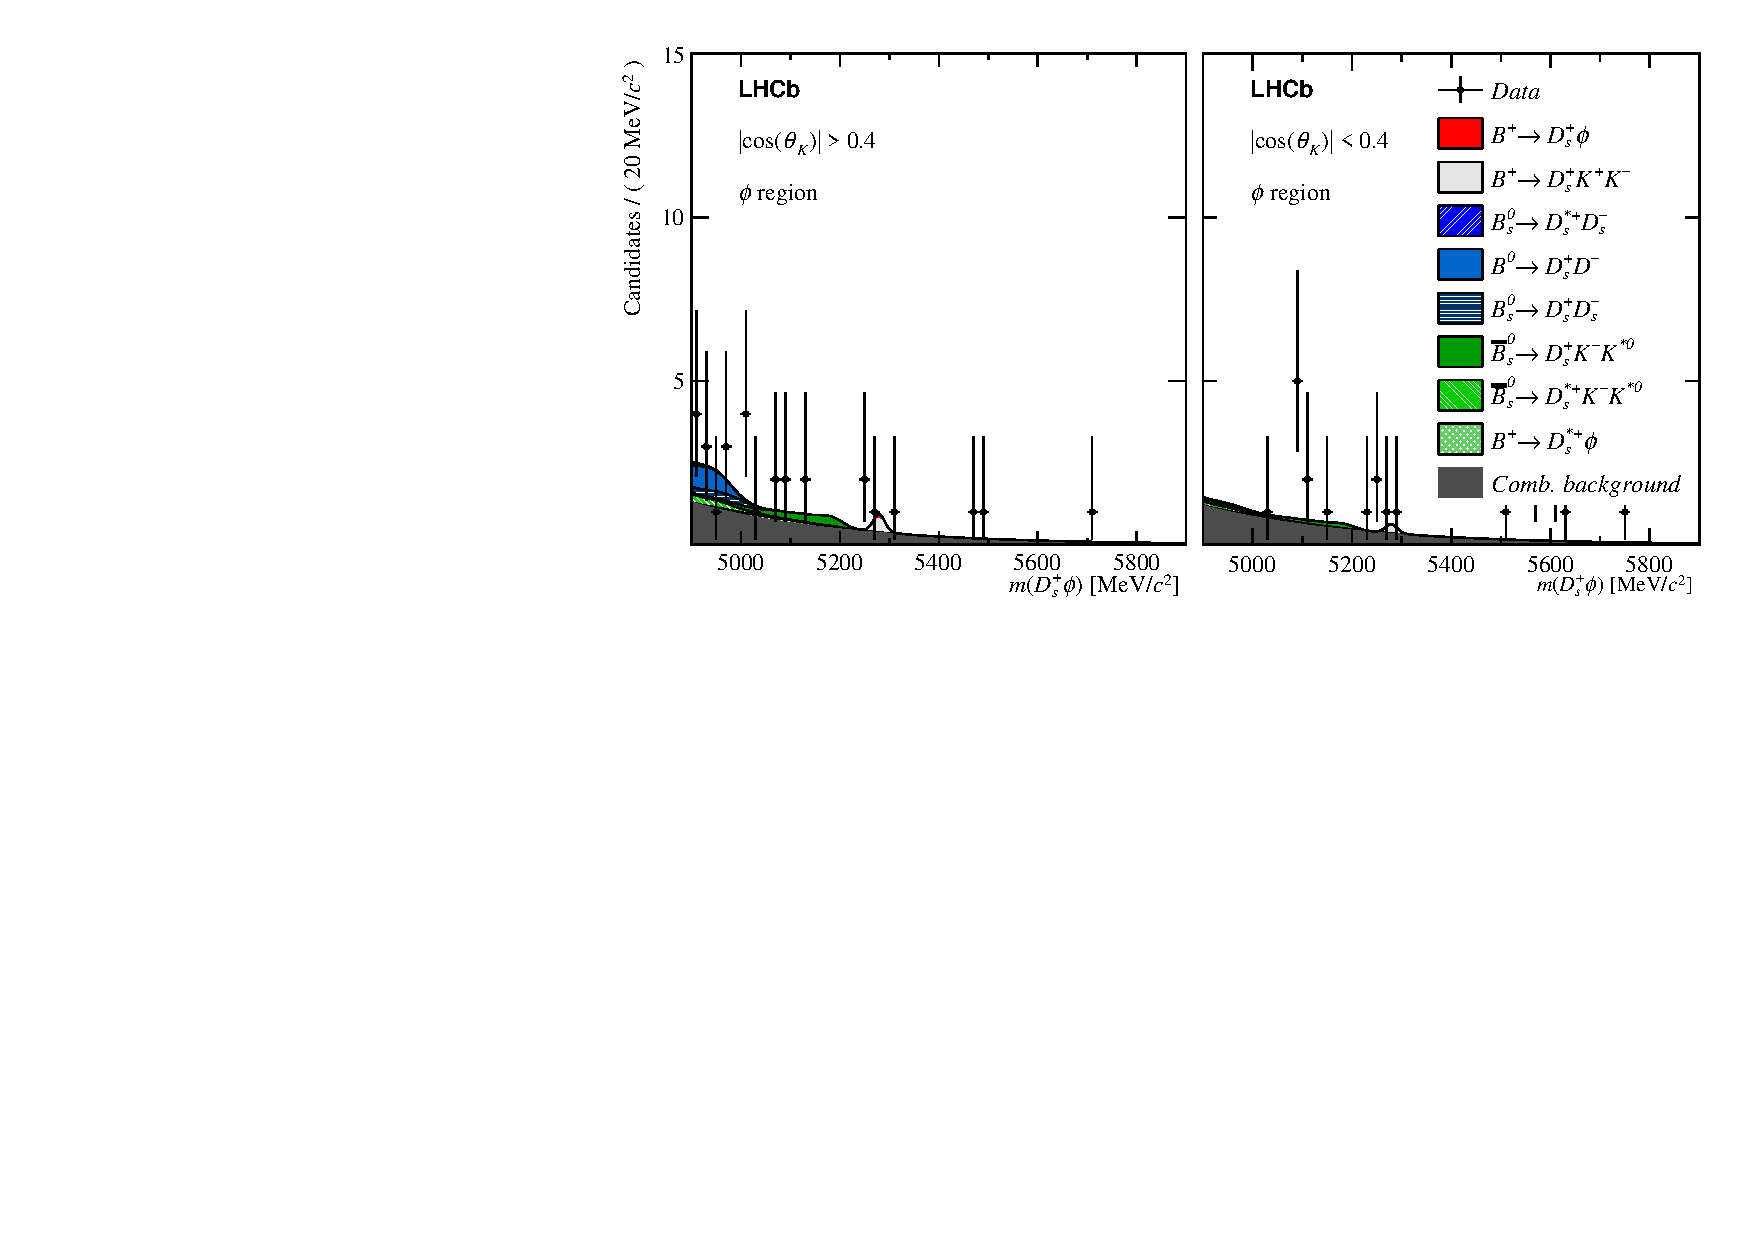
\includegraphics[width=0.7\textwidth]{figs/Appendix_FitCategories/canvas_DsPhi_Ds2KPiPi_both_summed_splitHel_splitKKPi_s21_s21r1_s24_s26.pdf}\\
        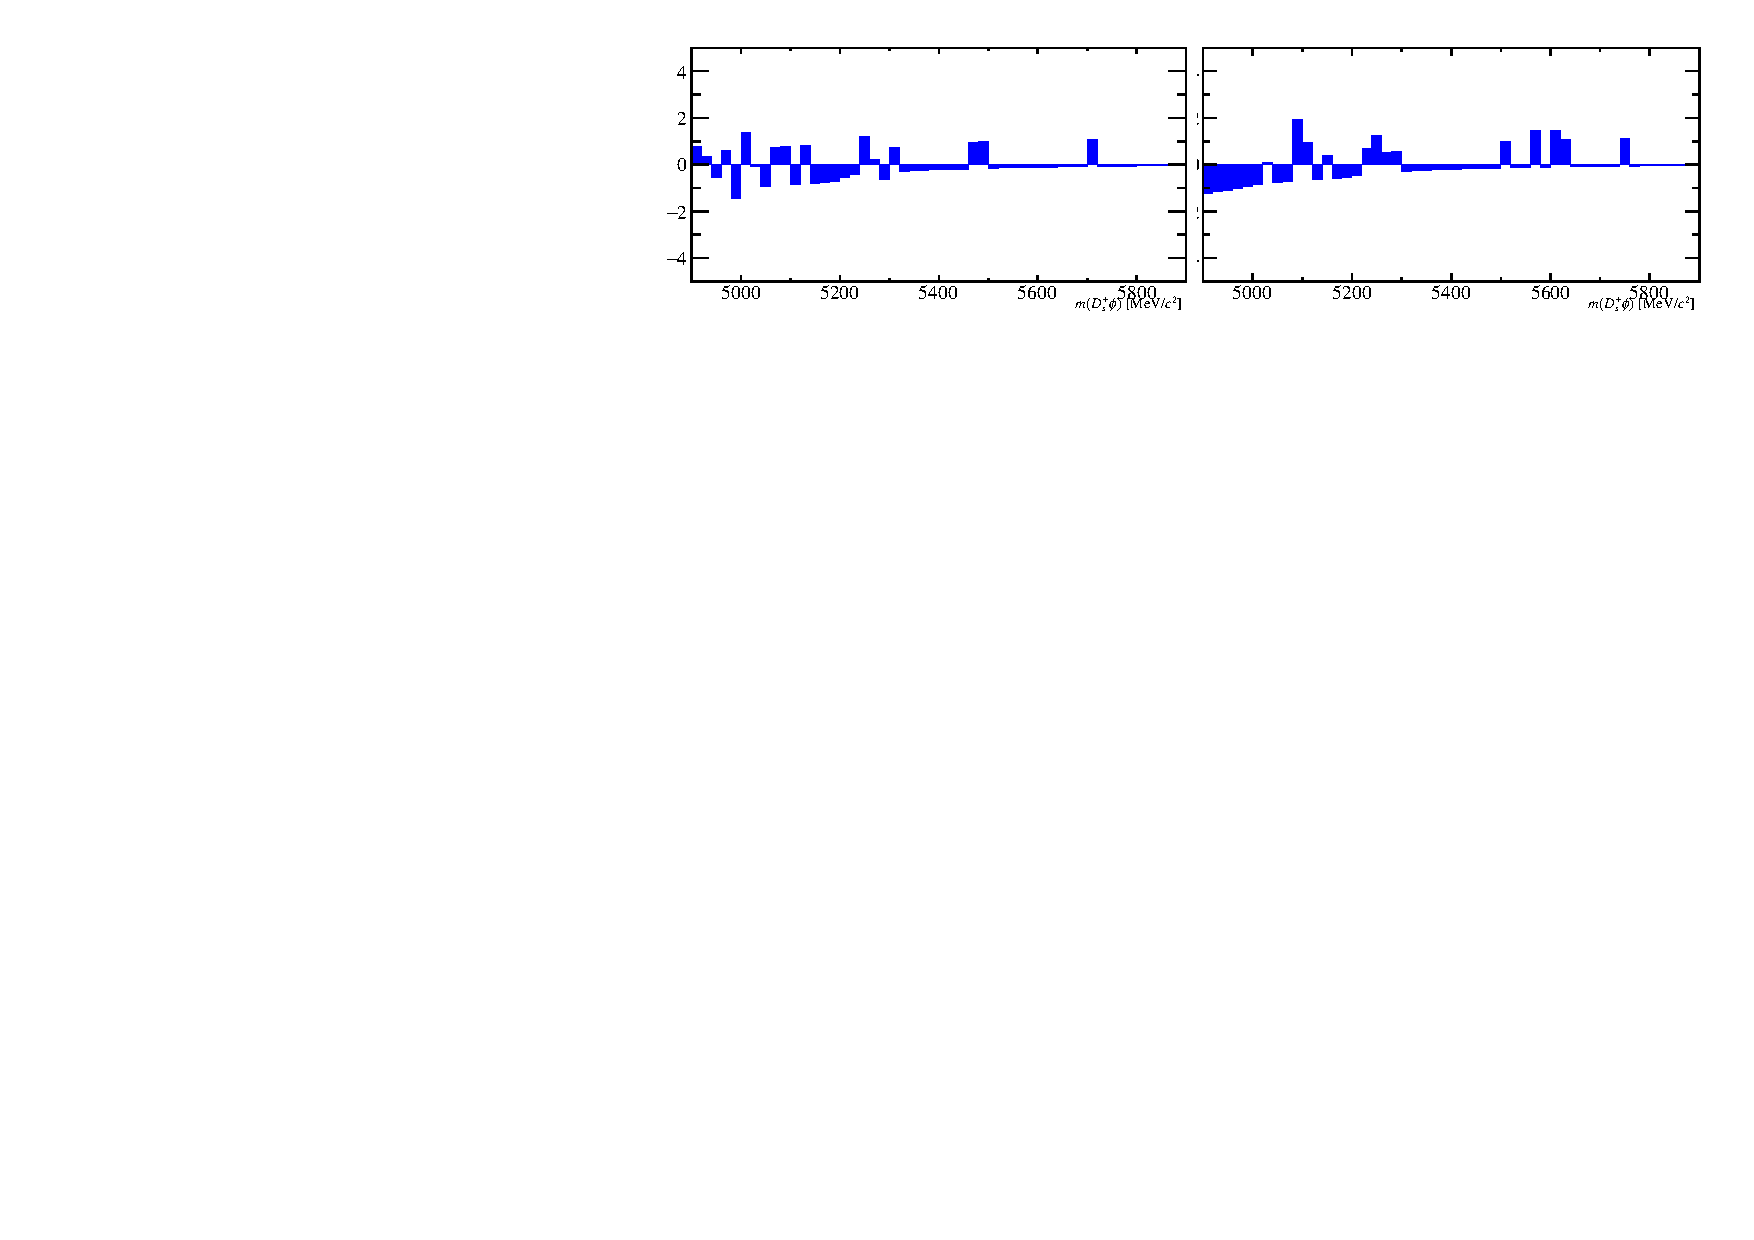
\includegraphics[width=0.7\textwidth]{figs/Appendix_FitCategories/residuals_DsPhi_Ds2KPiPi_both_summed_splitHel_splitKKPi_s21_s21r1_s24_s26.pdf}
    \end{subfigure}
    \begin{subfigure}[t]{1.0\textwidth}
        \centering
        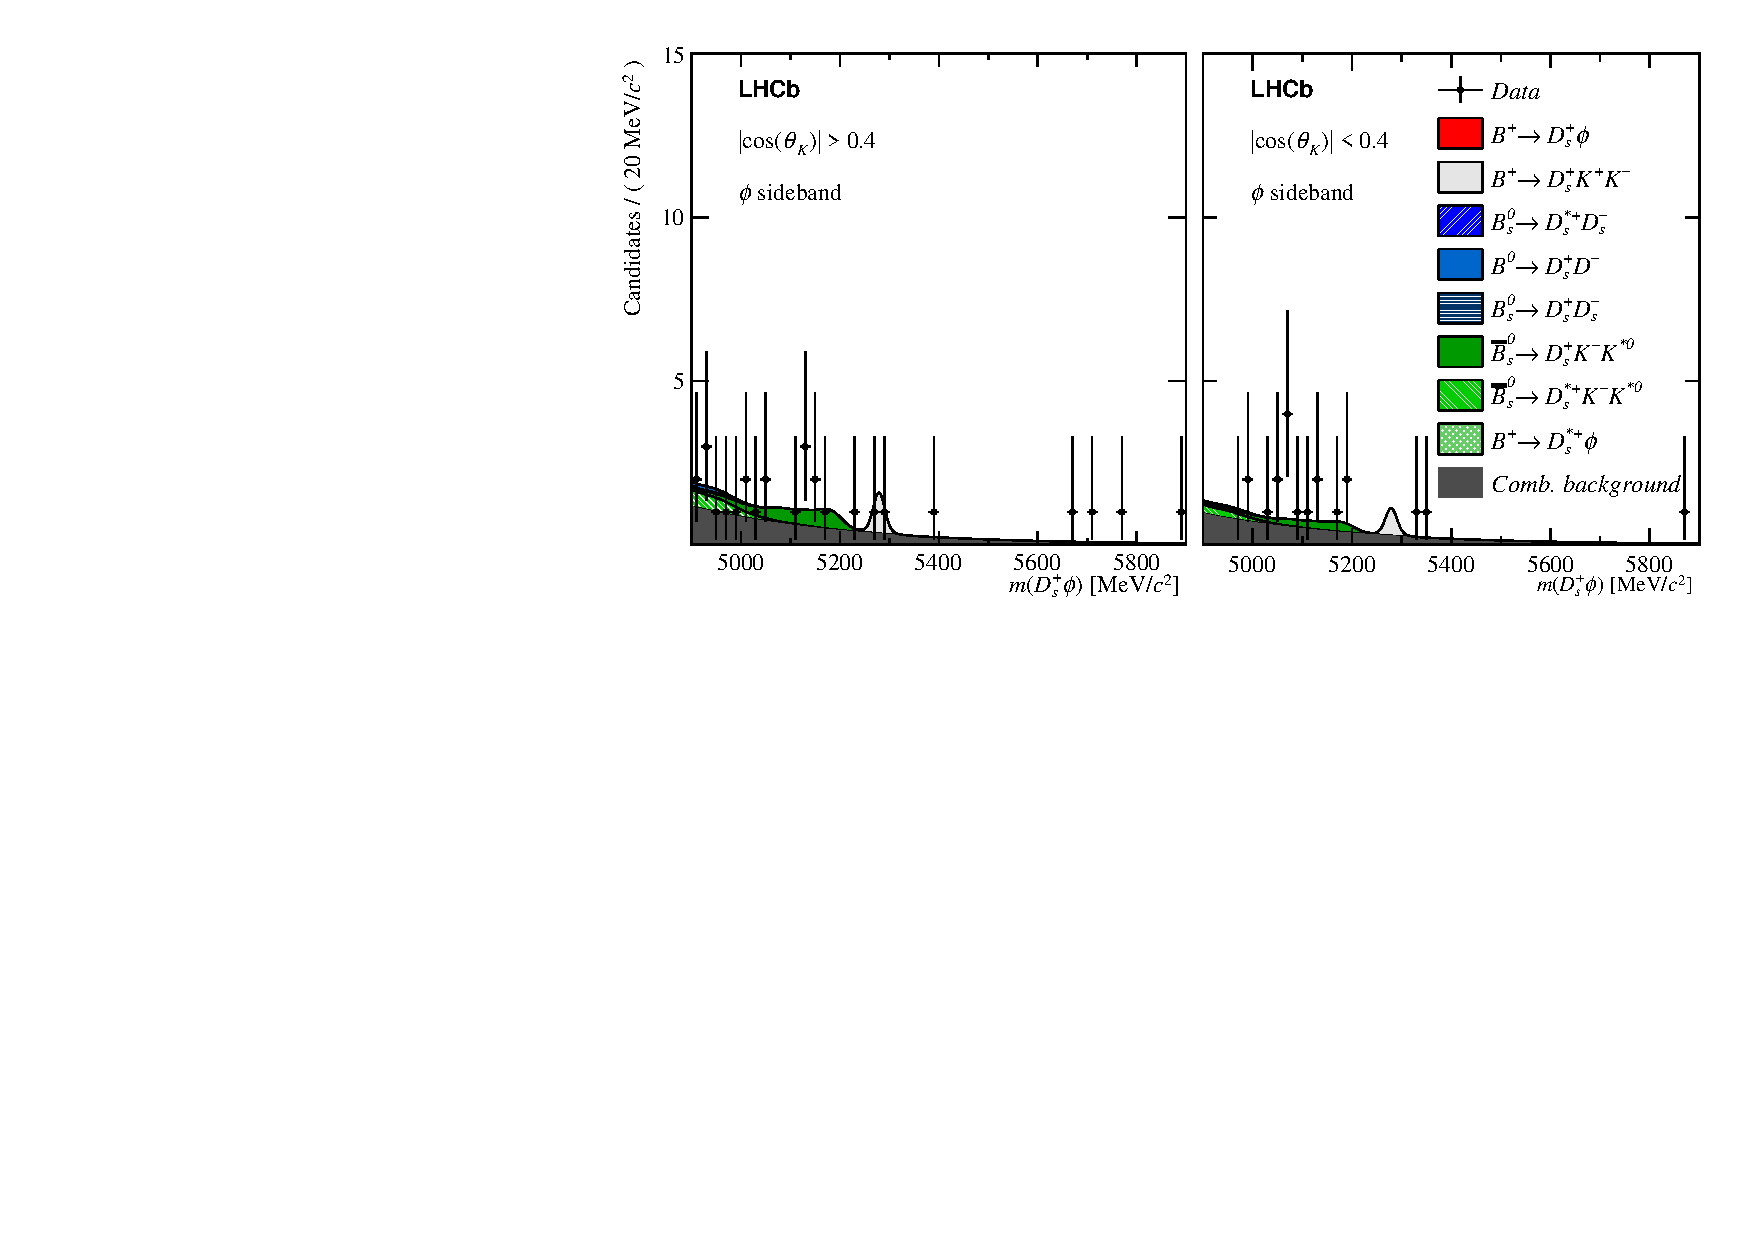
\includegraphics[width=0.7\textwidth]{figs/Appendix_FitCategories/canvas_DsPhiSide_Ds2KPiPi_both_summed_splitHel_splitKKPi_s21_s21r1_s24_s26.pdf}\\
        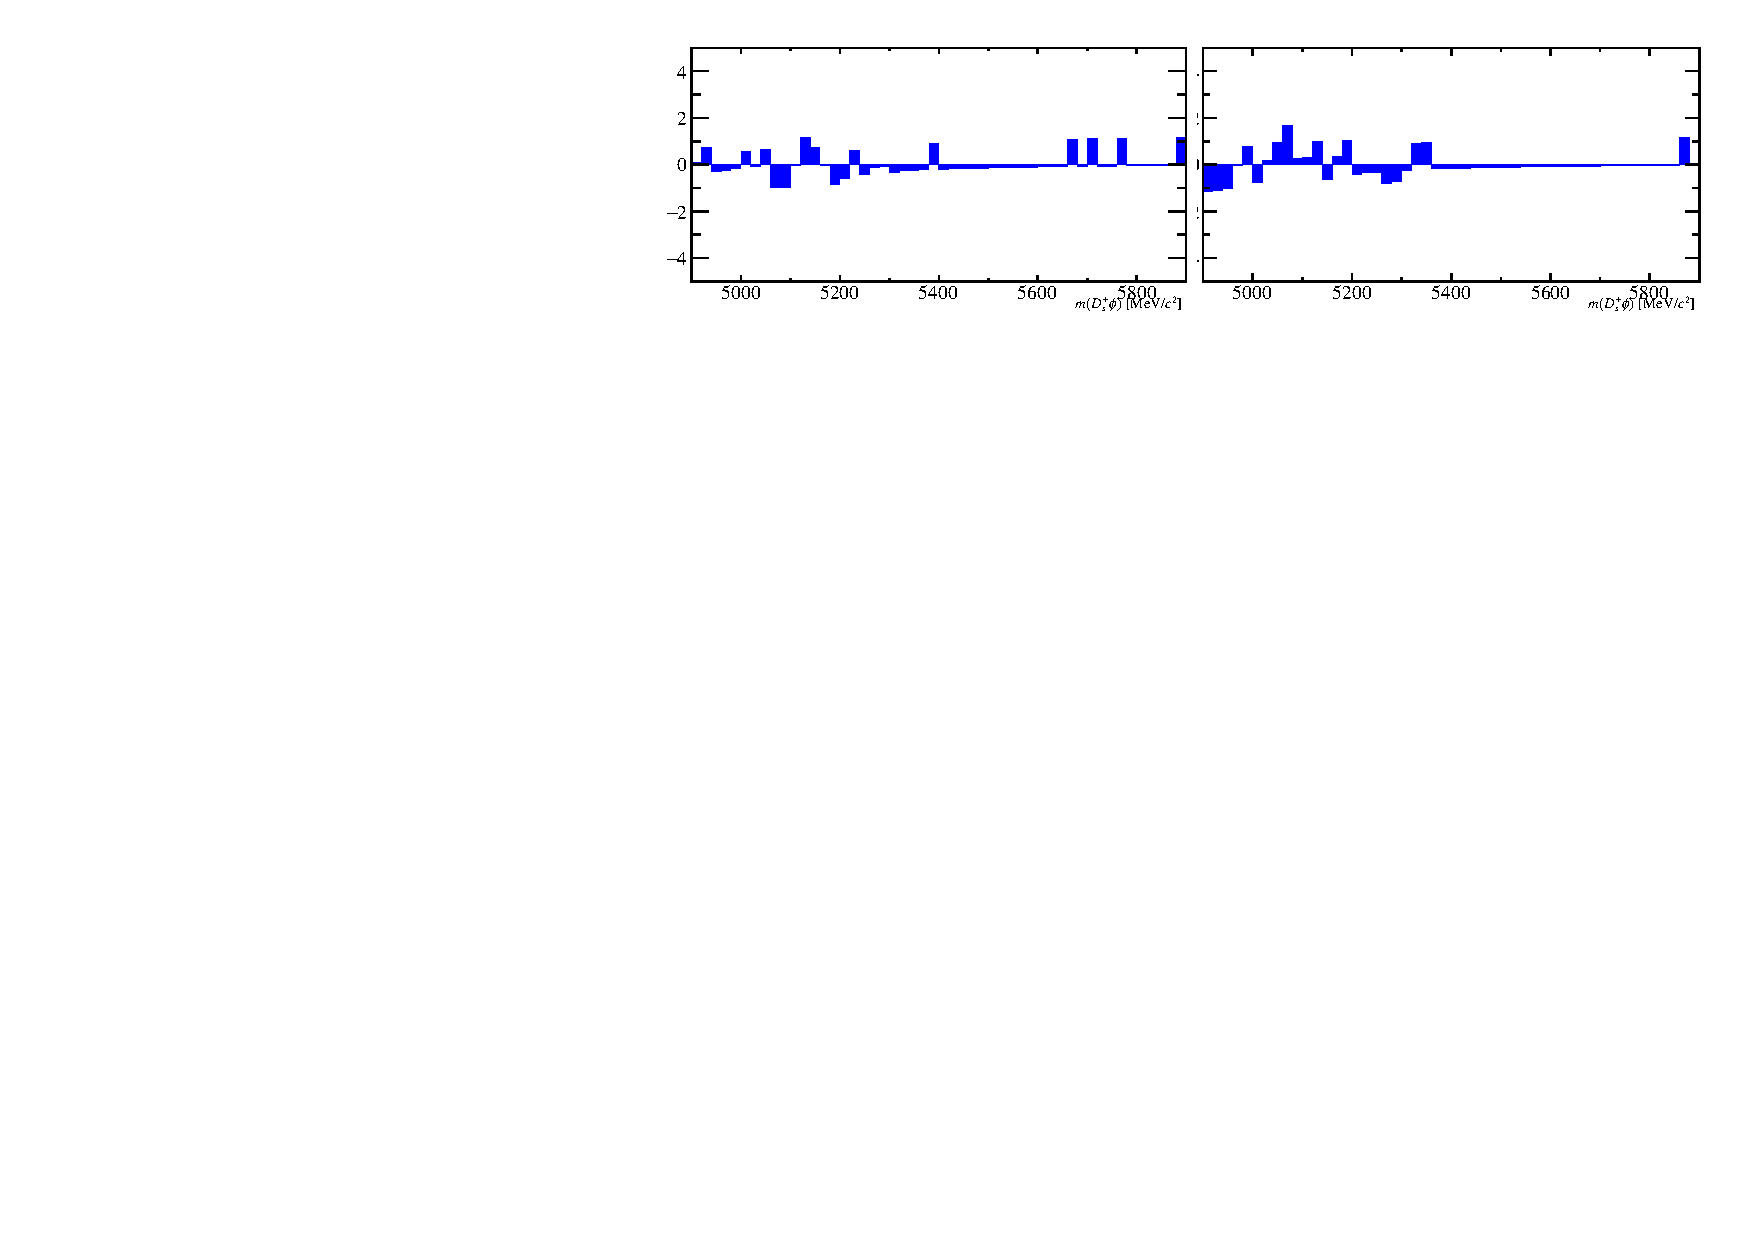
\includegraphics[width=0.7\textwidth]{figs/Appendix_FitCategories/residuals_DsPhiSide_Ds2KPiPi_both_summed_splitHel_splitKKPi_s21_s21r1_s24_s26.pdf}
    \end{subfigure}
    \caption{Invariant mass fits to \decay{\Bp}{\Dsp\phiz} candidates with \decay{\Dsp}{\Kp\pim\pip}.}
\end{figure}
%%%%%%%%%%%%%%%%%%%%%%%%%%%%%%%%%%%%%%%%%%%%%%%%%%%%%%%%%%

